\chapter{Methodologies}\label{chap:methodologies}

This section presents the methodologies applied to solve the \gls{cbrp} in its deterministic
and stochastic versions (\gls{scbrp}),
to simulate the spread of the Dengue virus, to develop a simulation-optimization framework
and for the statistical analysis of the results.

\section{Lagrangean Relaxations}\label{sec:lagrangean-relaxations}

\newcommand{\mult}[2]{\ensuremath{\lambda^{#1}_{#2}}}
\newcommand{\lrsp}{\textit{LR-SP}}
\newcommand{\lrkn}{\textit{LR-KN}}
\newcommand{\lrcsp}{\textit{LR-RCSP}}
\newcommand{\lrcspkn}{\textit{LR-RCSP-KN}}

This section presents the \gls{lr} obtained from the formulation Walk-CBRP, presented in
Section~\ref{sec:cbrp-walk-based-formulation}.
The Lagrange multipliers are represented by $\lambda$'s,
then~\mult{\ref{eq:walk-in-path}}{} and
\mult{\ref{eq:walk-max-time}}{} are
the non-negative variables  associated with the constraints~\eqref{eq:walk-in-path},
\eqref{eq:walk-max-time}, respectively. All  the relaxations have as their
\gls{lpp}, the \gls{kn}, \gls{sp} or the \gls{rcsp} subproblems.
The nomenclature used for each relaxation  follows the \gls{lr}-X pattern, where ``X''
represents one of the most difficult subproblems of the \gls{lpp} being solved.

\subsection{Lagrangean Relaxation with Shortest Path}\label{sec:lr-sp}

The \gls{lr} resulting from the dualization of the constraints~\eqref{eq:walk-in-path}
and~\eqref{eq:walk-max-time}
is very close to the problem of computing \gls{sp}s and is therefore called {\lrsp}.
The constraints~\eqref{eq:walk-s-t-all}-\eqref{eq:walk-flow-conservation}
and~\eqref{eq:walk-subtour-elimination}-\eqref{eq:walk-dom-y} model a problem similar
to create a path going from the depot $s = 0$ through the nodes of $V$ and going back to $s$,
using the variables $x_{ij}$ for all $i, j \in V, i \neq j$. As the \gls{lpp} contains no
constraint that apply to the variables $y_{b}$, the subproblem associated with these variables
consists in selecting the blocks $b \in B$ with the highest value  according to the lagrangian costs.
When the constraints~\eqref{eq:walk-in-path} and~\eqref{eq:walk-max-time}
are dualized, the resulting \gls{lpp} is:

\begin{align}
	\text{(LR-SP)}                                                                                                                                                \max \sum_{b \in B} p_{b} y_{b} + \mult{\ref{eq:walk-max-time}}{}
	(T - (\sum_{a \in A} x_{i,j}t_{i,j} + \sum_{b \in B} y_b t_b))                                                                                                & \label{eq:lrsp-of}   \\
	\nonumber                                                                                                                                                     + \sum_{b \in B} \mult{\ref{eq:walk-in-path}}{b}
	(\sum_{i \in V(b)} \sum_{a \in \delta^{-}(i)}x_{i,j} - y_b)                                                                                                   &                    & \\
	\nonumber \text{subject to: } \eqref{eq:walk-s-t-all}-\eqref{eq:walk-flow-conservation}\text{ and } \eqref{eq:walk-subtour-elimination}-\eqref{eq:walk-dom-y} &                    &
\end{align}


Thus, rearranging the terms, splitting into variables and inverting the signal in the X
term we have to solve the following optimization problems:
\begin{align}
	\text{(Y)}         & \max \sum_{b \in B} y_{b} (p_b - \mult{\ref{eq:walk-in-path}}{b} - \mult{\ref{eq:walk-max-time}}{} t_b) +                                                            \\
	\text{(X)}         & \max \sum_{(i,j) \in A} x_{i,j} \mult{\ref{eq:walk-max-time}}{} t_{i,j} - \sum_{b \in B} \sum_{(i,j) \in \delta^{+}(V(b))} x_{i,j} \mult{\ref{eq:walk-in-path}}{b} + \\
	\text{(constants)} & \mult{\ref{eq:walk-max-time}}{} T
\end{align}

Two approaches were used to solve {\lrsp}:  the first solution strategy is to use
an \gls{ilp}  solver to obtain  solutions in  each iteration of  the subgradient
method;  the  second  approach  is  to solve  the  \gls{lpp}  subproblems  using
combinatorial  algorithms.  A factor  that  influences  the complexity  of
solving  the  \gls{sp}  problem  is  related  to  the  possibility  of  negative
coefficients associated  with the variables  $x_{i,j}$ as consequence  of the
dualization of constraint~\eqref{eq:walk-max-time}.  Indeed, when  computing a
\gls{sp} the returned  solution may contain negative cycles, and  to avoid these
situations we define other variations of {\lrsp} by increasing the difficulty
of the subproblem adding time constraints.

\subsection{Lagrangean Relaxations with Time Constraints}\label{sec:lr-time-constraints}

Since the time constraint \eqref{eq:walk-max-time} is dualized and the resulting
\gls{lpp} is a \gls{sp} problem for variables $x_{i,j}$ and a selection problem for variables $y_b$,
we can define other variations of {\lrsp} by increasing the difficulty of the subproblem.
Thus, we increase the formulation Walk-CBRP by adding two new constraints that are redundant:
\begin{align}
	\sum_{(i,j) \in A} x_{i,j}t_{i,j} \leq T & \label{eq:arc-time-constraints}   \\
	\sum_{b \in B} y_b t_b \leq T            & \label{eq:block-time-constraints}
\end{align}

Thus, the resulting \gls{lpp}, referred as {\lrcsp}, is the variation of {\lrsp} with the addition of
Constraint~\eqref{eq:arc-time-constraints}.
The most difficult subproblem in the \gls{lpp} passes from a \gls{sp} problem to a
\gls{sp} problem with resource constraints, known as \gls{rcsp}. Since the amount
of time spent on the arcs is limited, the presence of negative costs not generate
a negative cycle that makes the subproblem infeasible. Computing  \gls{rcsp} is NP-hard,
however there are  exact algorithms that are efficient to  solve this problem in
practice~\cite{irnich:2006}. Our  implementations use  the labeling  algorithm
available  in   the  Boost  C++  Library~\cite{boost:2020}.

If the constraint~\eqref{eq:arc-time-constraints} is replaced by
the constraint~\eqref{eq:block-time-constraints}, the resulting \gls{lpp} will be referred as {\lrkn}.
The difficult subproblem in the \gls{lpp} now is associated with the variables $y_b$, that changes
from a selection problem to a \gls{kn} problem~\cite{karp:1972}. Computing a solution for the \gls{kn} problem
is NP-hard~\cite{korte:2008}, however there are exact algorithms based on dynamic programming that are
efficient to solve this problem in practice.

The most difficult version of this set of \gls{lrs} is {\lrcspkn}, tha uses both
constraints~\eqref{eq:arc-time-constraints} and~\eqref{eq:block-time-constraints}.
The resulting subproblems in the \gls{lpp} are \gls{kn} and \gls{rcsp} problems.
This relaxation is the expensive one in terms of computational demand.

\section{Deterministic \gls{cbrp} Heuristic}\label{sec:deterministic-heuristics}

This section present the heuristic approaches to solve the \gls{cbrp} in its deterministic version. The constructive heuristic of section~\ref{sec:greedy-constructive-algorithm} is a generic approach that can be used to solve the \gls{cbrp} also in its stochastic version.

\newcommand{\Call}[2]{\textit{#1}(#2)}

\subsection{Greedy Constructive Algorithm}\label{sec:greedy-constructive-algorithm}

The Greedy Constructive algorithm combines a binary search strategy to determine a high-quality time allocation with a \gls{kn}-based block selection and a heuristic routing method based on shortest paths in a \gls{dag}. The algorithm operates within three main steps: initially selects blocks to attend maximizing the profit per block, then defines a sequence for visiting all blocks of the previous step and, finally, create a route connecting those blocks in the selected order and check if it is feasible within the total time constraint.

\begin{algorithm}[h!]
	\caption{Greedy Constructive Algorithm}
	\SetAlgoLined
	\KwData{Graph $G$, time limit $T$}
	\KwResult{Solution with objective value $OF$, attended blocks $y$ and route $x$}

	\tcp{Initialization}
	$B \leftarrow$ number of blocks\;
	$y \leftarrow$ empty vector of blocks\;
	$x \leftarrow$ empty vector of arcs\;
	$OF \leftarrow 0$\;

	\tcp{Block Selection}
	\For{$i = 1$ \textbf{to} $B$}{
	$blocks[i] \leftarrow i$\;
	$time[i] \leftarrow$ time to attend block $i$\;
	$p_b[i] \leftarrow$ profit of block $i$\;
	}

	$OF \leftarrow$ \Call{SolveScenario}{$p_b$, $time$, $T$, $y$}\;

	\Return{$(OF, y, x)$}\;
\end{algorithm}

The SolveScenario routine implements a binary search strategy to find a good allocation of time between block attendance and routing. The algorithm starts by initializing the binary search bounds, with the lower bound $lb$ set to $0.5$ and upper bound $ub$ set to $1.0$, representing the fraction of total time $T$ that can be allocated to block attendance. The algorithm first attempts to find a solution using the full time budget $T$ by calling BinarySolve with $available\_time = T$. If this succeeds (returning a non-negative objective value), the algorithm immediately returns this as an optimal solution based on Property~\ref{property:knapsack-optimal-allocation}.

\begin{property}[Optimality of Knapsack Block Selection with Full Time Allocation]
	When the knapsack problem is used to select blocks with the total time budget $T$, and if the selected blocks can be connected by any feasible route respecting the time limit $T$, then the solution produced by the knapsack is optimal for the \gls{cbrp}.

	\begin{proof}
		The classical 0-1 knapsack problem maximizes the total profit
		(here, the number of cases attended) subject to a total time constraint $T$. The greedy heuristic first solves this knapsack problem to select a subset of blocks whose total time does not exceed $T$ and whose total profit is maximized. If, after this selection, exist at least one possible route to connect the selected blocks within the total time respecting the limit $T$, then there are no additional constraints beyond the knapsack constraint. Therefore, the solution found by the knapsack is not only feasible but also optimal for the \gls{cbrp}, as no other selection of blocks can yield a higher profit without exceeding the time limit. Thus, under the assumption of feasible routing, the knapsack solution is optimal.
	\end{proof}
	\label{property:knapsack-optimal-allocation}
\end{property}

If the full time allocation is infeasible, then the algorithm tries a more conservative approach by allocating only $50\%$ of the total time to block attendance. If this also fails, it adjusts the search bounds by setting the upper bound to the current lower bound and the lower bound to $0.0$, effectively searching in the range $[0.0, 0.5]$. If the $50\%$ allocation succeeds, it becomes the current best solution and the search continues in the range $[0.5, 1.0]$.

The binary search loop continues until the search interval becomes sufficiently small (less than $0.001$). In each iteration, the algorithm calculates the midpoint of the current search interval and attempts to solve the problem with that time allocation. If the solution is infeasible (BinarySolve returns \textit{infeasible}), the upper bound is reduced to the current midpoint. If feasible, the solution becomes the new best solution and the lower bound is increased to the current midpoint. This process efficiently define the most profitable feasible time allocation for block attendance and routing to connect the selected blocks.

\begin{algorithm}[h!]
	\caption{SolveScenario}
	\SetAlgoLined
	\KwData{block profit $p_b$, time limit $T$}
	\KwResult{Objective value $OF$}

	$lb \leftarrow 0.5$, $ub \leftarrow 1.0$, $mid \leftarrow 0.0$\;
	$OF \leftarrow 0$, $temp\_OF \leftarrow 0$\;
	$available\_time \leftarrow T$\;

	$temp\_OF \leftarrow$ \Call{BinarySolve}{$p_b$, $available\_time$, $T$, $y$}\;
	\If{$temp\_OF \text{is not \textit{infeasible}}$}{
		\Return{$temp\_OF$}; \tcp{Optimal solution}

	}

	$available\_time \leftarrow \lfloor 0.5 \times T \rfloor$; \tcp{Lower bound solution}
	$temp\_OF \leftarrow$ \Call{BinarySolve}{$p_b$, $available\_time$, $T$, $y$}\;
	\If{$temp\_OF \text{is \textit{infeasible}}$}{
		$ub \leftarrow lb$, $lb \leftarrow 0.0$\;
	}\Else{
		$OF \leftarrow temp\_OF$\;
	}
	$mid \leftarrow \frac{(lb + ub)}{2.0}$\;

	\tcp{Binary search loop}
	\While{$ub - lb > 0.001$}{
		$available\_time \leftarrow \lfloor mid \times T \rfloor$\;
		$temp\_OF \leftarrow$ \Call{BinarySolve}{$p_b$, $available\_time$, $T$, $y$}\;
		\If{$temp\_OF = -1$}{
			$ub \leftarrow mid$\;
		}\Else{
			$OF \leftarrow temp\_OF$, $y \leftarrow temp\_y$, $lb \leftarrow mid$\;
		}
		$mid \leftarrow \frac{(lb + ub)}{2.0}$\;
	}

	\Return{$OF$}\;
\end{algorithm}

The BinarySolve routine combines \gls{kn} optimization with routing feasibility checking to determine the optimal block selection for a given reserved time. The \gls{kn} solution selects the blocks that maximize the total profit within the available time. If no blocks can be selected (empty solution), the algorithm returns \textit{infeasible}. The block connection could use a caching mechanism based on the sequence of blocks to avoid redundant computations. The HeuristicBlockConnection routine is called to generate a route connecting the selected blocks in the sequence. Finally, the algorithm performs a feasibility check by verifying if the sum of block attendance time and the connecting routing time does not exceed the total time limit $MT$. If feasible, it returns the objective value, otherwise it returns \textit{infeasible}.

\begin{algorithm}[h!]
	\caption{BinarySolve}
	\SetAlgoLined
	\KwData{Block profit $p_b$, reserved time $reserved\_time$, maximum time $MT$}
	\KwResult{Objective value $OF$}

	$OF, y \leftarrow$ \Call{KnapsackSolve}{$p_b$, $reserved\_time$, $MT$}\;
	\If{$y$ is empty}{
		\Return{\textit{infeasible}}\;
	}

	$block\_attended\_time \leftarrow 0$; \tcp{Total attendance time}
	\For{each block $b$ in $y$}{
		$block\_attended\_time \leftarrow block\_attended\_time +$ time to attend block $b$\;
	}

	$connection\_time \leftarrow$ \Call{HeuristicBlockConnection}{$G$, $y$}; \tcp{Route time}

	\If{$block\_attended\_time + connection\_time \leq MT$}{
		\Return{$OF$}; \tcp{Feasible solution}
	}
	\Return{\textit{infeasible}}\;
\end{algorithm}

The KnapsackSolve routine implements the classic 0-1 \gls{kn} problem using \gls{dp}. The problem is formulated as selecting a subset of blocks that maximizes the total profit while respecting the time constraint. The algorithm initializes a two-dimensional \gls{dp} table $dp[n+1][MT+1]$ where $dp[i][w]$ represents the maximum profit that can be achieved using the first $i$ blocks with a time capacity of $w$. The table is initialized with zeros, representing the base case where no blocks are selected.

The \gls{dp} table is filled using the standard \gls{kn} recurrence relation. For each block $i$ and time capacity $w$, the algorithm considers two options: either include block $i$ (if its time requirement fits within the remaining capacity) or exclude it. The optimal choice is the one that maximizes the total profit. The recurrence relation is: $dp[i][w] = \max(dp[i-1][w], dp[i-1][w-time[i-1]] + p_b[i-1])$ if $time[i-1] \leq w$, otherwise $dp[i][w] = dp[i-1][w]$. This ensures that each block is considered at most once and the time constraint is respected.

After filling the \gls{dp} table, the algorithm backtracks to reconstruct the actual solution. Starting from the maximum time capacity $MT$ and the last block $n$, it checks if including block $i$ contributed to the optimal solution by comparing $dp[i][w]$ with $dp[i-1][w]$. If they differ, block $i-1$ is added to the solution and the remaining capacity is reduced accordingly.

\begin{algorithm}[h!]
	\caption{KnapsackSolve}
	\SetAlgoLined
	\KwData{block profit $p_b$, reserved time $T$}
	\KwResult{Maximum profit $OF$ and selected blocks $y$}

	$n \leftarrow$ number of blocks\;
	Initialize $dp[n+1][T+1]$ with zeros\;

	\For{$i = 1$ \textbf{to} $n$}{
		\For{$w = 1$ \textbf{to} $T$}{
			\If{$time[i-1] \leq w$}{
				$dp[i][w] \leftarrow \max(dp[i-1][w], dp[i-1][w-time[i-1]] + p_b[i-1])$\;
			}\Else{
				$dp[i][w] \leftarrow dp[i-1][w]$\;
			}
		}
	}

	\tcp{Backtrack to find selected blocks}
	$w \leftarrow T$\;
	\For{$i = n$ \textbf{downto} $1$}{
		\If{$dp[i][w] \neq dp[i-1][w]$}{
			Add block $i-1$ to $y$\;
			$w \leftarrow w - time[i-1]$\;
		}
	}

	\Return{$dp[n][T]$, $y$}\;
\end{algorithm}

The Algorithm~\ref{alg:heuristic-block-connection}, HeuristicBlockConnection, solves the routing problem for visiting all selected blocks using a greedy approach. This is essentially a variant of the \gls{tsp} where the goal is to find a minimum cost route that visits at least one node from all selected blocks. The algorithm first handles the trivial case where only one block is selected. In this case, no routing is needed, so the cost is zero and the path simply goes from the depot to any node of the block and back to the depot.

Besides the sequence of blocks, the heuristic defines the route that connects those blocks and which node attends to each block. The algorithm uses an approach that variates the sequence of blocks (sorting option) and the distance considered between the blocks (the smallest shortest path between each pair of blocks or the shortest path between a specific node from the current block and a specific node of the next block). The algorithm sort the blocks to be attended according to the sorting option and the distance criteria for the greedy heuristic, then create a multi-layered \gls{dag}, that will be described in more details next in this section, to compute the shortest route that visits all blocks in $\mathcal{B}'$. The shortest route is then computed by finding the shortest path from the artificial depot $s$ to $t$ in the \gls{dag}. The route time is then calculated by summing the time of the arcs in the path and the algorithm maintains the best solution found across all the 8 combinations of $sort\_opt$ and $block\_distance\_opt$.

\begin{algorithm}[h!]
	\caption{Heuristic Block Connection}\label{alg:heuristic-block-connection}
	\SetAlgoLined
	\KwData{Graph $G$, shortest path calculator $SP$, selected blocks $blocks$}
	\KwResult{best route time $best\_time$ and route $best\_path$}

	\If{$|blocks| = 1$}{
		\Return{$0$}; \tcp{Single block}
	}
	$best\_time \leftarrow \infty$\;
	$best\_path \leftarrow$ empty\;

	\For{$block\_distance\_opt = 1$ \textbf{to} $2$}{
		\For{$sort\_opt = 1$ \textbf{to} $4$}{
			$ordered\_blocks \leftarrow$ \Call{GreedyBlockOrderingHeuristic}{$blocks$, $sort\_opt$, $block\_distance\_opt$}\;
			$G_{DAG} \leftarrow$ \Call{CreateLayeredDAG}{$ordered\_blocks$}\;
			$path \leftarrow$ \Call{ShortesPathInDAG}{$G_{DAG}(s, t)$}\;
			$time \leftarrow$ \Call{CalculateTime}{$path$}\;
			\If{$time < best\_time$}{
				$best\_time \leftarrow time$\;
				$best\_path \leftarrow path$\;
			}
		}
	}
	\Return{$best\_time$, $best\_path$}\;
\end{algorithm}

The Algorithm~\ref{alg:greedy-block-ordering-heuristic} presents a greedy heuristic that determines the order in which the blocks must be visited. Given a set of blocks $\mathcal{B} = \{b_1, b_2, \ldots, b_m\}$, a sorting option $sort\_opt$, and a block distance option $block\_distance\_opt$, the algorithm constructs an ordered sequence $\mathcal{B}' = \{b'_1, b'_2, \ldots, b'_m\}$ that iteratively minimizes the total travel distance between consecutive blocks. The parameter $sort\_opt$ contains the following options:

\begin{itemize}
	\item When $sort\_opt = 0$, blocks are sorted in ascending order by the cummulative hops of the block nodes. Hops are the number of arcs in the shortest path between a node $i \in V$ and the closest node $j \in V$ of the block $b \in B$ in the Graph $G$. The goal here is to prioritize blocks that are, in general, closer to the higher number of other blocks in the graph.
	\item When $sort\_opt = 1$, blocks are sorted in descending order by the number of nodes they contain, favoring larger blocks that offer more routing flexibility.
	\item When $sort\_opt = 2$, blocks are sorted by their count of zero-hop nodes in descending order, emphasizing blocks with high internal connectivity.
	\item When $sort\_opt = 3$, blocks are shuffled randomly.
\end{itemize}

And two options for the block distance option $block\_distance\_opt$:
\begin{itemize}
	\item When $block\_distance\_opt = \text{B2B}$, the distance between blocks is the lowest shortest path between all nodes from block $b_1$ to nodes in block $b_2$.
	\item When $block\_distance\_opt = \text{N2B}$, the distance between blocks is the shortest path between a specific node from the current block and all nodes in the next block.
\end{itemize}

Following the initial sorting, the algorithm employs a strategy to iteratively construct the block visitation sequence. The first block in the sorted list is selected as the starting point, and a reference node from this block is identified as having the minimum distance to the next unvisited block in the sorted list. In subsequent iterations, the algorithm evaluates all unvisited blocks and selects the one within the shortest path from the current reference node. When multiple blocks have equal distances, ties are broken by preferring blocks with larger numbers of nodes, as these provide greater flexibility in path construction. The reference node is then updated to the closest node in the newly selected block, and this process continues until all blocks have been used.

Given an ordered sequence of blocks $\mathcal{B} = \{b_1, b_2, \ldots, b_m\}$ to visit, the next step is to construct a multi-layered \gls{dag} where each layer $i$ corresponds to block $b_i$ and contains a new vertex for each node that belongs to the block in the original graph $G$. The formal definition of the \gls{dag} is $G_{DAG} = (V_{DAG}, A_{DAG})$ where $V_{DAG} = \{s, t\} \cup v^{b_i}_k: i \in \mathcal{B}, k \in V(b_i)$ and $A_{DAG} = \{(s, v^{b_1}_{k}), (v^{b_m}_{k'}, t): k \in V(b_1), k' \in V(b_m)\} \cup \{(v^{b_i}_o, v^{b_{i+1}}_{d}): i = 1, \ldots, m-1, o \in V(b_i), d \in V(b_{i+1})\}$.  The weight of each arc $(i, j) \in A_{DAG}$ is the shortest path distance between the nodes $i$ and $j$ in the graph $G$ Each path from $s$ to $t$ in $G_{DAG}$ include at least one node from each block in $\mathcal{B}$.

Figure~\ref{fig:layered-dag-adaptation} presents an example of the adaptation for the layered-dag. The graph $G$ in represented in Figure~\ref{subfig:original-graph}, that contains the blocks $A$, $B$ and $C$. Considering that those blocks must be visited in the order $\mathcal{B}': A \rightarrow C \rightarrow B$, the resulting graph $G_{DAG}$ is presented in Figure~\ref{subfig:layered-dag}. One possible solution is presented in Figure~\ref{subfig:layered-dag-solution}, using node $11$ to attend blocks $A$ and $C$, and node $6$ to attend block $B$. The $G_{DAG}$ solution is $s \rightarrow A_{11} \rightarrow C_{11} \rightarrow B_{6} \rightarrow t$, that could be mapped to the original graph as $s \rightarrow 11 \rightarrow 8 \rightarrow 6 \rightarrow t$. The route connecting $s$ and $t$ could be obtained by using any shortest path algorithm.

\begin{figure}[h!]
	\centering
	\begin{minipage}[c]{.45\textwidth}
		\begin{tikzpicture}[
				> = stealth, % arrow head style
				shorten > = 0.8pt, % don't touch arrow head to node
				auto,
				node distance = 2cm, % distance between nodes
				semithick % line style
			]

			\tikzstyle{every state}=[
			draw = black,
			thick,
			fill = white,
			minimum size = 8mm
			]

			\node[state] (a) at (0,0) {$1$};
			\node[state, right of = a] (b) {$2$};
			\node[state, above of = a] (c) {$3$};
			\node[state, draw = white, text=teal, below of = c, right of = a, yshift=3cm, xshift=-1cm] {A};

			\node[state, right of = b, xshift=0.1cm] (d) {$4$};

			\node[state, right of = d, xshift=0.1cm] (e) {$5$};
			\node[state, above of = d, xshift=0.1cm] (f) {$6$};
			\node[state, above of = e] (g) {$7$};
			\node[state, draw = white, text=red, above of = e, right of = f, yshift=-2.6cm, xshift=-0.6cm] {B};

			\node[state, above of = f, xshift=-0.3cm] (h) {$8$};
			\node[state, above of = h] (i) {$9$};
			\node[state, left of = i] (j) {$10$};
			\node[state, below of = j] (k) {$11$};
			\node[state, draw = white, text=green, below of = j, right of = k, yshift=3cm, xshift=-1cm] {C};

			\path[->] (a) edge node {} (c);
			\path[->] (c) edge node {} (a);

			\path[->] (k) edge node {} (b);
			\path[->] (b) edge node {} (k);

			\path[->] (k) edge node {} (c);
			\path[->] (c) edge node {} (k);

			\path[->] (b) edge node {} (a);
			\path[->] (a) edge node {} (b);

			\path[->] (b) edge node {} (d);
			\path[->] (d) edge node {} (b);

			\path[->] (d) edge node {} (e);
			\path[->] (e) edge node {} (d);

			\path[->] (e) edge node {} (f);
			\path[->] (f) edge node {} (e);

			\path[->] (f) edge node {} (g);
			\path[->] (g) edge node {} (f);

			\path[->] (g) edge node {} (e);
			\path[->] (e) edge node {} (g);

			\path[->] (h) edge node {} (k);
			\path[->] (k) edge node {} (h);

			\path[->] (k) edge node {} (j);
			\path[->] (j) edge node {} (k);

			\path[->] (j) edge node {} (i);
			\path[->] (i) edge node {} (j);

			\path[->] (i) edge node {} (h);
			\path[->] (h) edge node {} (i);

			\path[->] (f) edge node {} (h);
			\path[->] (h) edge node {} (f);

		\end{tikzpicture}
		\subcaption{\label{subfig:original-graph} Original Graph $G$.}
	\end{minipage}
	\\
	\begin{minipage}[c]{.45\textwidth}
		\begin{tikzpicture}[
				> = stealth, % arrow head style
				shorten > = 0.8pt, % don't touch arrow head to node
				auto,
				node distance = 1.5cm, % distance between nodes
				semithick % line style
			]

			\tikzstyle{every state}=[
			draw = black,
			thick,
			fill = white,
			minimum size = 11mm
			]

			\node[state, double] (s) at (0,0) {$s$};
			\node[state, right of = s, draw = white] (depot_legend) {Depot};

			\node[state, below of = s, draw = teal, xshift=-0.6cm, yshift=-0.5cm] (a2) {$A_2$};
			\node[state, left of = a2, draw = teal] (a1) {$A_1$};
			\node[state, right of = a2, draw = teal] (a3) {$A_3$};
			\node[state, right of = a3, draw = teal] (a11) {$A_{11}$};

			\node[state, below of = a1, yshift=-1cm, draw = green] (c8) {$C_8$};
			\node[state, right of = c8, draw = green] (c9) {$C_9$};
			\node[state, right of = c9, draw = green] (c10) {$C_{10}$};
			\node[state, right of = c10, draw = green] (c11) {$C_{11}$};

			\node[state, below of = c9, xshift=-0.8cm, yshift=-1cm, draw = red] (b5) {$B_5$};
			\node[state, right of = b5, draw = red] (b6) {$B_6$};
			\node[state, right of = b6, draw = red] (b7) {$B_7$};

			\node[state, double, below of = b6, yshift=-0.5cm] (t) {$t$};
			% Arcs
			\path[->, draw=black, thick] (s) edge (a1);
			\path[->, draw=black, thick] (s) edge (a2);
			\path[->, draw=black, thick] (s) edge (a3);
			\path[->, draw=black, thick] (s) edge (a11);

			\path[->, draw=black, thick] (a1) edge (c8);
			\path[->, draw=black, thick] (a1) edge (c9);
			\path[->, draw=black, thick] (a1) edge (c10);
			\path[->, draw=black, thick] (a1) edge (c11);
			\path[->, draw=black, thick] (a2) edge (c8);
			\path[->, draw=black, thick] (a2) edge (c9);
			\path[->, draw=black, thick] (a2) edge (c10);
			\path[->, draw=black, thick] (a2) edge (c11);
			\path[->, draw=black, thick] (a3) edge (c8);
			\path[->, draw=black, thick] (a3) edge (c9);
			\path[->, draw=black, thick] (a3) edge (c10);
			\path[->, draw=black, thick] (a3) edge (c11);
			\path[->, draw=black, thick] (a11) edge (c8);
			\path[->, draw=black, thick] (a11) edge (c9);
			\path[->, draw=black, thick] (a11) edge (c10);
			\path[->, draw=black, thick] (a11) edge (c11);

			\path[->, draw=black, thick] (c8) edge (b5);
			\path[->, draw=black, thick] (c8) edge (b6);
			\path[->, draw=black, thick] (c8) edge (b7);
			\path[->, draw=black, thick] (c9) edge (b5);
			\path[->, draw=black, thick] (c9) edge (b6);
			\path[->, draw=black, thick] (c9) edge (b7);
			\path[->, draw=black, thick] (c10) edge (b5);
			\path[->, draw=black, thick] (c10) edge (b6);
			\path[->, draw=black, thick] (c10) edge (b7);
			\path[->, draw=black, thick] (c11) edge (b5);
			\path[->, draw=black, thick] (c11) edge (b6);
			\path[->, draw=black, thick] (c11) edge (b7);

			\path[->, draw=black, thick] (b5) edge (t);
			\path[->, draw=black, thick] (b6) edge (t);
			\path[->, draw=black, thick] (b7) edge (t);

			% \path[->, draw = gray, opacity = 0.2] (a) edge node {} (c);
			% \path[->, draw = gray, opacity = 0.2] (c) edge node {} (b);
			% \path[->, draw = gray, opacity = 0.2] (b) edge node {} (a);

			% \path[->, draw = black, opacity = 1.0, dashed] (b) edge node {} (d);
			% \path[->, draw = black, opacity = 1.0, dashed] (d) edge node {} (e);

			% \path[->, draw = black, opacity = 1.0, dashed] (e) edge node {} (f);
			% \path[->, draw = gray, opacity = 0.2] (f) edge node {} (g);
			% \path[->, draw = gray, opacity = 0.2] (g) edge node {} (e);

			% \path[->, draw = gray, opacity = 0.2] (h) edge node {} (k);
			% \path[->, draw = gray, opacity = 0.2] (k) edge node {} (j);
			% \path[->, draw = gray, opacity = 0.2] (j) edge node {} (i);
			% \path[->, draw = gray, opacity = 0.2] (i) edge node {} (h);

			% \path[->, draw = black, opacity = 1.0, dashed] (f) edge node {} (h);
		\end{tikzpicture}
		\subcaption{\label{subfig:layered-dag} Layered DAG $G_{DAG}$.}
	\end{minipage}
	\hfill
	\begin{minipage}[c]{.45\textwidth}
		\begin{tikzpicture}[
				> = stealth, % arrow head style
				shorten > = 0.8pt, % don't touch arrow head to node
				auto,
				node distance = 1.5cm, % distance between nodes
				semithick % line style
			]

			\tikzstyle{every state}=[
			draw = black,
			thick,
			fill = white,
			minimum size = 11mm
			]

			\node[state, double] (s) at (0,0) {$s$};
			\node[state, right of = s, draw = white] (depot_legend) {Depot};

			\node[state, below of = s, draw = teal, xshift=-0.6cm, yshift=-0.5cm] (a2) {$A_2$};
			\node[state, left of = a2, draw = teal] (a1) {$A_1$};
			\node[state, right of = a2, draw = teal] (a3) {$A_3$};
			\node[state, right of = a3, draw = teal] (a11) {$A_{11}$};
			% \node[state, right of = a11, draw = white] (depot_legend) {Block A};

			\node[state, below of = a1, yshift=-1cm, draw = green] (c8) {$C_8$};
			\node[state, right of = c8, draw = green] (c9) {$C_9$};
			\node[state, right of = c9, draw = green] (c10) {$C_{10}$};
			\node[state, right of = c10, draw = green] (c11) {$C_{11}$};
			% \node[state, right of = c11, draw = white] (depot_legend) {Block C};

			\node[state, below of = c9, xshift=-0.8cm, yshift=-1cm, draw = red] (b5) {$B_5$};
			\node[state, right of = b5, draw = red] (b6) {$B_6$};
			\node[state, right of = b6, draw = red] (b7) {$B_7$};
			% \node[state, right of = b7, draw = white] (depot_legend) {Block B};

			\node[state, double, below of = b6, yshift=-0.5cm] (t) {$t$};
			% Arcs
			\path[->, draw=gray, opacity=0.2, thick] (s) edge (a1);
			\path[->, draw=gray, opacity=0.2, thick] (s) edge (a2);
			\path[->, draw=gray, opacity=0.2, thick] (s) edge (a3);
			\path[->, draw=black, thick] (s) edge (a11);

			\path[->, draw=gray, opacity=0.2, thick] (a1) edge (c8);
			\path[->, draw=gray, opacity=0.2, thick] (a1) edge (c9);
			\path[->, draw=gray, opacity=0.2, thick] (a1) edge (c10);
			\path[->, draw=gray, opacity=0.2, thick] (a1) edge (c11);
			\path[->, draw=gray, opacity=0.2, thick] (a2) edge (c8);
			\path[->, draw=gray, opacity=0.2, thick] (a2) edge (c9);
			\path[->, draw=gray, opacity=0.2, thick] (a2) edge (c10);
			\path[->, draw=gray, opacity=0.2, thick] (a2) edge (c11);
			\path[->, draw=gray, opacity=0.2, thick] (a3) edge (c8);
			\path[->, draw=gray, opacity=0.2, thick] (a3) edge (c9);
			\path[->, draw=gray, opacity=0.2, thick] (a3) edge (c10);
			\path[->, draw=gray, opacity=0.2, thick] (a3) edge (c11);
			\path[->, draw=gray, opacity=0.2, thick] (a11) edge (c8);
			\path[->, draw=gray, opacity=0.2, thick] (a11) edge (c9);
			\path[->, draw=gray, opacity=0.2, thick] (a11) edge (c10);
			\path[->, draw=black, thick] (a11) edge (c11);

			\path[->, draw=gray, opacity=0.2, thick] (c8) edge (b5);
			\path[->, draw=gray, opacity=0.2, thick] (c8) edge (b6);
			\path[->, draw=gray, opacity=0.2, thick] (c8) edge (b7);
			\path[->, draw=gray, opacity=0.2, thick] (c9) edge (b5);
			\path[->, draw=gray, opacity=0.2, thick] (c9) edge (b6);
			\path[->, draw=gray, opacity=0.2, thick] (c9) edge (b7);
			\path[->, draw=gray, opacity=0.2, thick] (c10) edge (b5);
			\path[->, draw=gray, opacity=0.2, thick] (c10) edge (b6);
			\path[->, draw=gray, opacity=0.2, thick] (c10) edge (b7);
			\path[->, draw=gray, opacity=0.2, thick] (c11) edge (b5);
			\path[->, draw=black, thick] (c11) edge (b6);
			\path[->, draw=gray, opacity=0.2, thick] (c11) edge (b7);

			\path[->, draw=gray, opacity=0.2, thick] (b5) edge (t);
			\path[->, draw=black, thick] (b6) edge (t);
			\path[->, draw=gray, opacity=0.2, thick] (b7) edge (t);
		\end{tikzpicture}
		\subcaption{\label{subfig:layered-dag-solution} Solution generated in $G_{DAG}$.}
	\end{minipage}
	\caption{\label{fig:layered-dag-adaptation} Layered DAG Adaptation.}
\end{figure}

\begin{algorithm}[h!]
	\caption{Greedy Block Ordering Heuristic}\label{alg:greedy-block-ordering-heuristic}
	\SetAlgoLined
	\KwData{Blocks to visit $\mathcal{B}$, sorting option $sort\_opt$, block distance option $block\_distance\_opt$}
	\KwResult{Ordered sequence $\mathcal{B}'$ of blocks}

	$\mathcal{B}' \leftarrow \emptyset$\;
	$backup\_blocks \leftarrow \mathcal{B}$\;

	\tcp{Apply initial sorting strategy}
	\uIf{$sort\_opt = 0$}{
		Sort $backup\_blocks$ by cumulative hops (ascending)\;
	}
	\uElseIf{$sort\_opt = 1$}{
		Sort $backup\_blocks$ by number of nodes in the blocks (descending)\;
	}
	\uElseIf{$sort\_opt = 2$}{
		Sort $backup\_blocks$ by zero-hop count (descending)\;
	}
	\uElse{
		Shuffle $backup\_blocks$\;
	}

	\tcp{Iterative block selection}
	\While{$|connect\_order| < |\mathcal{B}|$}{
		\uIf{$\mathcal{B}'$ is empty}{
			Add first block from $backup\_blocks$ to $\mathcal{B}'$\;
			Find reference node with minimum distance to next block\;
		}

		$best\_block \leftarrow -1$, $min\_distance \leftarrow \infty$\;
		\For{each candidate block $b$ in $backup\_blocks$}{
			\uElseIf{$block\_distance\_opt = \text{B2B}$}{
				$(distance, ref\_node) \leftarrow \Call{MinBlock2BlockTime}{last\_ref\_block, b}$\;
			}
			\uElse {
				$(distance, ref\_node) \leftarrow$ \Call{MinNode2BlockTime}{$last\_ref\_node, b$}\;
			}
			$num\_nodes \leftarrow$ number of nodes in block $b$\;
			\If{$distance < min\_distance$ \textbf{or} ($distance = min\_distance$ \textbf{and} $num\_nodes > num\_best\_nodes$)}{
				$min\_distance \leftarrow distance$\;
				$best\_block \leftarrow b$\;
				$best\_ref\_node \leftarrow ref\_node$\;
			}
		}
		Add $best\_block$ to $\mathcal{B}'$\;
		Remove $best\_block$ from $backup\_blocks$\;
		$last\_ref\_node \leftarrow best\_ref\_node$\;
		$last\_ref\_block \leftarrow best\_block$\;

	}
	\Return{$\mathcal{B}'$}\;
\end{algorithm}

\section{Stochastic \gls{cbrp} Heuristics}\label{sec:stochastic-heuristics}

This section presents the stochastic heuristics for the \gls{cbrp}. The heuristics are divided into three main sections: constructive, local search and a metaheuristic based on simulated annealing.

The first step is to highlight the similarities between the deterministic and stochastic versions of the \gls{cbrp}. Considering the formulation Path-SCBRP, presented in Section~\ref{sec:cbrp-stochastic-models}, the first relevant property is that the stochastic version of the problem is a set of $k = |S|$ independent \gls{cbrp} instances, one for each scenario $s \in S$ considering a fixed first stage solution. Therefore, it is possible to use deterministic approaches to solve stages and scenarios independently.

\begin{figure}[h!]
	\centering
	\begin{tikzpicture}
		[
			node distance=1.9cm, % distance between nodes
			font=\tiny,
			align=center
		]

		% Defining styles
		\tikzstyle{startstop} = [rectangle, rounded corners, minimum width=3cm, minimum height=1cm, text centered, draw=black, text width=3cm, fill=blue!30!white]

		%%%%%%%%%%%%%%%%%%%%%%%%%%%%%%%%%%%%%%%%%%%%%%%%%%%%%%%%%%%%%%%%%%%%%%%

		\tikzstyle{io} = [ellipse, minimum width=2cm, text width=2cm, minimum height=1cm, text centered, draw=black, fill=gray!30!white, font=\bf\tiny]

		\tikzstyle{process} = [tape, minimum width=1.5cm, text width=2cm, minimum height=1cm, text centered, draw=black, fill=green!30!white, font=\bf\tiny]

		\tikzstyle{decision} = [diamond, text width=1.5cm, aspect=2, text height=1, text centered, draw=black, fill=yellow!30!white, font=\bf\tiny]

		\tikzstyle{stage} = [rectangle, minimum width=1cm, text width=1cm, minimum height=1cm, draw=black, font=\bf\tiny]

		\tikzstyle{artificial} = [rectangle, draw=white, font=\bf\tiny]

		\tikzstyle{arrow} = [thick,->,>=stealth]

		% Create states
		\node (start) [process] at (0, 0) {Greedy Deterministic Heuristic\\for each scenario};

		\node (ls_in_route) [process, below of=start, xshift=-5cm] {In Route Swap};
		\node (ls_out_route) [process, right of=ls_in_route, xshift=1cm] {Out Route Swap};
		\node (ls_add_block) [process, right of=ls_out_route, xshift=1cm] {Add Block to Route};
		\node (ls_remove_block) [process, right of=ls_add_block, xshift=1cm] {Remove Block from Route};
		\node (ls_route_improvement) [process, right of=ls_remove_block, xshift=1cm] {Route Improvement};

		\node (swap_random) [startstop, below of=ls_route_improvement, xshift=-5cm] {Swap Random Block};
		\node (swap_first) [startstop, right of=swap_random, xshift=1cm] {Swap First Improve};
		\node (swap_best) [startstop, right of=swap_first, xshift=1cm] {Swap Best Improve};



		% \node (deterministic) [startstop, right of=start, xshift=7cm] {Deterministic\\Optimization\\Problem};

		% % Links
		% \draw [arrow] (start) -- node[text width=3cm, fill=white, align=center] {Replacement of Random Elements} (deterministic);

		% %%%%%%%%%%%%%%%%%%%%%%%%%%%%%%% Stage 1 %%%%%%%%%%%%%%%%%%%%%%%%%%%%%%
		% %%%%%%%%%%%%%%%%%%%%%%%%%%%%%%%%%%%%%%%%%%%%%%%%%%%%%%%%%%%%%%%%%%%%%%
		% \node (metaheuristic) [process, below of=deterministic] {Metaheuristic Algorithm};

		% \node (deterministic-sol) [io, below of=metaheuristic] {New Deterministic Solution};
		% \node (ml-component) [process, below of=deterministic-sol] {Machine Learning Component};
		% \node (fast-sim-component) [process, below of=ml-component] {Fast Simulation Component};

		% \node (promissing-sol) [decision, xshift=-2.5cm, left of=ml-component] {Promissing\\Solution?};
		% \node (surrogate-sol) [decision, xshift=-2.5cm, left of=fast-sim-component] {Surrogate\\Model\\Available?};

		% \node (surrogate-component) [process, below of=surrogate-sol] {Surrogate Model};

		% \node (update-sol-list) [io, below of=surrogate-component] {Update Solution List};

		% \node (available-time) [decision, xshift=-2.5cm, left of=update-sol-list] {Available\\Computation\\Time?};

		% % Links
		% \draw [arrow] (deterministic) -- (metaheuristic);
		% \draw [arrow] (metaheuristic) -- (deterministic-sol);
		% \draw [arrow] (deterministic-sol) -- (ml-component);

		% \draw [arrow] (ml-component) -- (promissing-sol);
		% \draw [arrow] (promissing-sol) -- node[anchor=east] {yes} (surrogate-sol);
		% \draw [arrow] (promissing-sol) -| node[anchor=south,xshift=2.5cm] {no} (available-time);

		% %
		% \draw [arrow] (surrogate-sol) -- node[anchor=east] {yes} (surrogate-component);
		% \draw [arrow] (surrogate-sol) -- node[anchor=north] {no} (fast-sim-component);

		% %
		% \draw [arrow] (surrogate-component) -- (update-sol-list);
		% \draw [arrow] (update-sol-list) -- (available-time);

		% % 
		% \draw [arrow] (available-time.west) |- node[anchor=west, yshift=-8.5cm] {yes} (metaheuristic);

		% % Feedback
		% \node (art1) [artificial, right of=metaheuristic, xshift=0.5cm] {};

		% \draw [arrow,dashed,-] (metaheuristic) -- (art1.center);
		% \draw [arrow,dashed] (art1.center) |- node[text width=1cm, fill=white, align=center, rotate=270, xshift=-1.8cm] {Feedback} (ml-component.north east);

		% % 
		% \node (art2) [artificial, right of=ml-component, xshift=0.5cm] {};

		% \draw [arrow,dashed,-] (ml-component.east) -- (art2.center);
		% \draw [arrow,dashed] (art2.center) |- node[text width=1cm, fill=white, align=center, rotate=270, xshift=-1.9cm] {Feedback} (surrogate-component);

		% % 
		% \node (art3) [artificial, right of=fast-sim-component] {};

		% \draw [arrow,dashed,-] (fast-sim-component.east) -- (art3.center);
		% \draw [arrow,dashed] (art3.center) |- node[text width=1cm, fill=white, align=center, rotate=270, xshift=0.8cm] {Feedback} (ml-component.south east);

		% \node (stage1) [stage, fit=(art1.east) (update-sol-list) (available-time) (deterministic-sol) (start.south west), yshift=-0.5cm] {};
		% \node (art4) [artificial, left of=stage1, rotate=90, yshift=5.5cm] {Stage 1};

		% % Second Stage
		% \node (elite-sol) [io, below of=available-time, yshift=-0.75cm] {Elite Stochastic Solutions};
		% \node (intensive-sim-component) [process, below of=update-sol-list, yshift=-0.75cm] {Intensive Simulation Component};

		% \draw [arrow] (available-time) -- node[anchor=east, yshift=0.5cm] {no} (elite-sol);
		% \draw [arrow] (elite-sol) -- (intensive-sim-component);

		% \node (art5) [artificial, left of=elite-sol, below of=available-time, xshift=0.3cm] {};
		% \node (art6) [artificial, right of=intensive-sim-component, below of=intensive-sim-component, yshift=1.25cm, xshift=4.9cm] {};

		% \node (stage2) [stage, fit=(art5) (art6)] {};
		% \node (art7) [artificial, left of=stage2, rotate=90, yshift=5.5cm] {Stage 2};

		% % Third stage
		% \node (risk-component) [process, below of=intensive-sim-component, yshift=-0.25cm] {Risk/Reliability\\Component};
		% \draw [arrow] (intensive-sim-component) -- (risk-component);

		% \node (art8) [artificial, left of=risk-component, below of=elite-sol, xshift=0.3cm, yshift=0.55cm] {};
		% \node (art9) [artificial, right of=risk-component, below of=risk-component, yshift=1.25cm, xshift=4.9cm] {};

		% \node (stage3) [stage, fit=(art8) (art9)] {};
		% \node (art10) [artificial, left of=stage3, rotate=90, yshift=5.5cm] {Stage 3};

		% % Final
		% \node (elite-stochastic-sol) [io, below of=risk-component, yshift=-0.5cm] {Elite Stochastic\\Solutions with Probabilistic Information};

		% \draw [arrow] (risk-component) -- (elite-stochastic-sol);
	\end{tikzpicture}
	\caption{Logic Behind Simheuristics \cite{juan:2022}.}
	\label{fig:logic-simheuristics}
\end{figure}

\subsection{Constructive Heuristic}

Considering that the first stage and the scenarios of the second stage could be solve independently, the initial solution for the \gls{scbrp} could use the constructive heuristic presented in Section~\ref{sec:greedy-constructive-algorithm}. More details about the constructive heuristic are presented in Section~\ref{sec:greedy-constructive-algorithm}.

The initial solution heuristic for the \gls{scbrp} is based on a two-stage approach that leverages deterministic greedy algorithms. In the first stage, all blocks are assigned adjusted profit values that combine both the nominal (first-stage) and scenario-based (second-stage) profits for each block, weighted by the reduction factor $\alpha$ and scenario probabilities. The greedy constructive algorithm is then used to generate a feasible first-stage route that maximizes the aggregated profit while respecting the time constraint. Subsequently, for each scenario, the algorithm solves an independent routing problem where the profits associated with first-stage-visited blocks are appropriately reduced, reflecting the fact that those blocks have already been serviced. The greedy constructive algorithm is applied to each scenario with these adjusted profit values, producing scenario-specific routes. The overall solution consists of the first-stage routing plan together with a collection of scenario-dependent second-stage routes, thus providing a complete and feasible plan for the \gls{scbrp}.

\begin{algorithm}[h!]
	\caption{Create Initial Solution}
	\SetAlgoLined
	\KwData{graph $G$, scenarios $S$, time limit $T$, blocks $B$, reduction factor $\alpha$, first-stage profit $p_b^{0}$, scenario profit $p_b^{\omega}$}
	\KwResult{Solution with first-stage route and scenario-specific routes}
	
	$solution \leftarrow \text{new Solution}(Input)$\;
	
	$cases\_per\_block \leftarrow \text{vector of size } |B|$\;
	$time\_per\_block \leftarrow \text{vector of size } B$\;
	
	\tcp{Set first-stage profit values for all blocks}
	\For{$b = 1$ \textbf{to} $|B|$}{
		$cases\_per\_block[b] \leftarrow p_{b}^{0} + \alpha \sum_{\omega \in \Omega} \xi^{\omega} p_{b}^{\omega}$\;	
	}

	\tcp{Solve first stage using greedy heuristic and add to solution}
	$first\_stage\_of \leftarrow \Call{GreedyConstructiveAlgorithm}{cases\_per\_block, T, y_0}$\;
	Add first-stage allocation and route to solution\;
	
	\tcp{Solve Second Stage Problems for each scenario}
	\For{$s = 1$ \textbf{to} $S$}{
		\tcp{Adjust scenario costs based on first-stage solution}
		\For{$b = 1$ \textbf{to} $|B|$}{
			\uIf{$y_b^{0} = 1$}{
				$cases\_per\_block[b] \leftarrow (1 - \alpha) p_{b}^{s}$\;
			}\Else{
				$cases\_per\_block[b] \leftarrow p_{b}^{s}$\;
			}
		}
		$scn\_of \leftarrow \Call{GreedyConstructiveAlgorithm}{cases\_per\_block, T, y_s}$\;
		Add scenario allocation and route to solution\;
		$scn\_of \leftarrow \xi^{s} \times scn\_of$\;
	}
	\Return{$solution$}\;
\end{algorithm}

\subsection{Local Search Heuristic}

\subsection{Simulated Annealing Heuristic}

\section{Dengue Virus Spread Simulation}\label{sec:dengue-virus-spread-simulation}

This section presents the design and implementation of the proposed \gls{mabs}
following the compartmental theory~\citep{amaku:2014}. The model adopts a SIR
compartment for human agents and SEI for mosquitoes. Birth and death rates are
considered for the mosquito population, while the human population remains
constant throughout all simulations. Transitions from susceptible to infected
(or exposed) occur based on interactions between a susceptible agent and an
infected agent of the opposite species.

Table~\ref{tab:parameters-mabs} presents the description of the model parameters
as well as their chosen values. Most parameter values are based on those
explored in the works of~\cite{da-silva:2020} and \cite{dwivedi:2022}. The other
parameters, especially those that established the generation of new mosquitoes,
are adjusted with experiments discussed in
Section~\ref{sec:computational-experiments}.

% Parameters
\begin{table}[!ht]
	\centering
	\caption{\label{tab:parameters-mabs} Static parameters used in the proposed
		\gls{mabs}.} \small{%
		\begin{tabular}{clr}
			\toprule
			\textbf{Parameter} & \textbf{Description}                                  & \textbf{Value} \\ \midrule
			$\gamma_H$         & Human recovery rate per day                           & 0.146          \\ \hline
			$a$                & Daily rate of bites                                   & 0.168          \\ \hline
			$b$                & Fraction of infectious bites                          & 0.600          \\ \hline
			$\gamma_M$         & Mosquito latency rate per day                         & 0.143          \\ \hline
			$c$                & Mosquito susceptibility to dengue                     & 0.526          \\ \hline
			$\rho$             & The percentage of eggs that produce female mosquitoes & 0.125
			\\ \hline
			$\phi$             & Mosquito daily oviposition rate                       & 0.020          \\ \hline
			$\omega$           & Carrying capacity of the mosquito                     & 3.000          \\
			\hline
			$\delta$           & Mosquito daily mortality rate in aquatic phase        & 0.066          \\ \hline
			$\sigma$           & Mosquito daily maturation rate                        & 0.100          \\ \hline
			$\mu_M$            & Mosquito daily mortality rate in adult phase          & 0.010
			\\ \hline
			$\Delta_M$         & Daily rate of eggs to female adult mosquitoes         &
			0.125                                                                                       \\
			\bottomrule
		\end{tabular}%
	}
\end{table}

Each value in Table~\ref{tab:parameters-mabs} represents the probability applied
to agents in the simulation in each cycle. The parameter $\gamma_H$ denotes the
likelihood of a human transitioning from Infected to Recovered. The parameter
$a$ indicates the chance of a human being bitten by a nearby mosquito, while $b$
represents the probability that a bite from an infected mosquito is infectious.
The transition of a mosquito from exposed to infected depends on $\gamma_M$. If
a mosquito bites an infected human, the probability of the mosquito becoming
infected is given by $c$. The parameter $\rho$ signifies the number of eggs that
hatch into female mosquitoes, $\phi$ is the likelihood of a mosquito laying eggs
due to an interaction with a breeding site, and $\omega$ represents the maximum
number of eggs deposited per interaction. The parameter $\delta$ indicates the
probability of an egg dying, while $\sigma$ is the probability of it developing
into an adult susceptible mosquito. Finally, $\mu_M$ is the adult mosquito
mortality rate.

\subsection{MABS Agents} \label{sec:agents}

The model has four types of agents that could have some interactions with each
other: mosquito, human, egg, and breeding site. The sizes of the human and
breeding site populations do not change during the simulation. The mosquito
agent is divided into two phases: aquatic and adult. The breeding site agent
represents a point on the map that allows mosquitoes to lay eggs to proliferate
new individuals for the population, independent of the current state. The
mosquitoes in the starting population and those generated during the simulation
are associated with a breeding site.

This work does not consider vertical transmission, i.e., mosquitoes do not
transmit the virus to eggs in the breeding sites. This information implies that
all mosquitoes changing from the aquatic to adult phase in a breeding site start
as susceptible. A simplified flowchart of interactions is presented in
Figure~\ref{fig:simplified-agent-interaction}, followed by a more detailed
description.

\begin{figure}[!ht]
	\begin{tikzpicture}[ node distance = 4.0cm, block/.style = {rectangle, draw,
					minimum width=2cm, minimum height=1cm, fill=lightgray, rounded corners,
					fill opacity=0.4, text=black, text opacity=1.0}, arrow/.style = {->,
					thick}, dashedarrow/.style = {->, thick, dashed}, dashedbox/.style =
				{draw, dashed, inner sep=10pt, rounded corners, opacity=0.2}
			% Define dashed box style
		]

		% Nodes
		\node (P) {Human}; \node [block, right of=P, xshift=-1cm] (S)
		{Susceptible}; \node [block, right of=S, xshift=1.5cm] (I) {Infected};
		\node [block, right of=I] (R) {Recovered};
		% \node[dashedbox, fit=(S) (I) (R)] (Box) {};

		% Arrows
		\draw [arrow] (S) -- (I) node[midway, above, color=black] {$1 - (1 - a
				\times b)^{n_{I}}$}; \draw [arrow] (I) -- (R) node[midway, above,
			color=black] {$\gamma_H$};

		\node [below of=P, yshift=2cm] (M) {Mosquitoes}; \node [block, right
			of=M, below of=P, yshift=2cm, xshift=-1cm] (SM) {Susceptible}; \node
		[block, right of=SM, below of=S, yshift=2cm, xshift=1.5cm] (EM)
		{Exposed}; \node [block, right of=EM, below of=I, yshift=2cm] (IM)
		{Infected};

		\node[dashedbox, fit=(SM) (EM) (IM)] (Box2) {};

		% Arrows
		\draw [arrow] (SM) -- (EM) node[midway, below, color=black] {$1 - (1 - a
				\times c)^{m_i}$}; \draw [arrow] (EM) -- (IM) node[midway, below,
			color=black] {$\gamma M$};

		\draw [dashedarrow, color=gray] (SM) -- (I) node[midway, above,
			color=black] {$a$}; \draw [dashedarrow, color=gray] (IM) -  - (S)
		node[midway, above, color=black] {$b$};

		%
		\node [below of=M, yshift=1cm] (AQ) {Aquatic Stage}; \node [block, right
			of=B, below of=M, yshift=1cm, xshift=-1cm] (EGG) {Egg};

		\node [block, right of=EGG, below of=SM, yshift=1cm, xshift=1.5cm] (BS)
		{Breeding Site};

		\draw [dashedarrow, color=gray] (Box2) -- (BS) node[midway, right,
			color=black] {$\omega$};

		\draw [dashedarrow, color=gray] (BS) -- (EGG) node[midway, above,
			color=black] {$(1 - \delta)$};

		\draw [dashedarrow, color=gray] (EGG) -- (SM) node[midway, left,
			color=black] {$(\sigma \times \rho)$};

		%
		% \node [below of=AQ, yshift=1cm] (BS) {Breeding Site:}; \node [block,
		% right of=BS, below of=EGG, yshift=1cm] (EGG) {Egg};
	\end{tikzpicture}

	\caption{Simplified agent interaction flowchart.}
	\label{fig:simplified-agent-interaction}
\end{figure}


\begin{itemize}
	\item \textbf{Human Agent:}
	      \begin{itemize}
		      \item \textbf{Location}: For each human, two blocks are randomly defined to
		            represent work and resting places. The exact point inside of each block is
		            also defined randomly.
		      \item \textbf{Move}: Considering the basic people's routines, they cycle
		            every day between two locations. It is assumed that humans have a residence
		            and a destination point, which may be, for example, school or work. The
		            movement is based on daily hours; each human has a ``$start\_work\_time$"
		            that is a time between 5 AM and 8 AM, indicating the time when the agent
		            starts to move from home to its destination, setting the current objective
		            to ``working". The ``$end\_work\_time$" follows the same pattern,
		            representing the return home between 4 PM and 7 PM, changing the current
		            objective to ``resting''.
		      \item \textbf{Change to Infected state}: Changing a human agent from
		            susceptible to infected requires interaction with infected mosquitoes. The
		            higher the number of infected mosquitoes nearby, the greater the chance of
		            this state transition. Assume $n_I$ as the number of infected mosquitoes
		            within a 1-meter distance and the probability of a human being infected by
		            the bite of an infected mosquito. From these values, consider $(a \times b)$
		            as the probability of a human becoming infected. Thus, the chance of
		            changing from a susceptible to an infected state is given by $1 - (1 - a
			            \times b)^{n_{I}}$.
		      \item  \textbf{Change to Recovered state}: Changing from infected to
		            recovered depends on the parameter $\gamma_H$.
	      \end{itemize}

	\item \textbf{Breeding Site Agent.}
	      \begin{itemize}
		      \item \textbf{Location}: Each breeding site is located at a random point
		            inside a street block.
		      \item \textbf{Create new eggs}: When a mosquito lays an egg at a breeding
		            site, this interaction creates a new Egg agent in the simulation. This new
		            egg is associated with the breeding site, and this decision impacts the
		            movement range of the adult mosquito.
	      \end{itemize}

	\item \textbf{Egg Agent.}
	      \begin{itemize}
		      \item \textbf{Location}: All Egg agents are located inside breeding sites.
		      \item \textbf{Change to  Adult phase}: The change from aquatic to adult
		            phase depends on the maturation rate ($\sigma$), and the successfully
		            hatched egg rate ($\rho$). The probability of an egg changing to the adult
		            stage is given by $\sigma \times \rho$.
		      \item \textbf{Aquatic Phase Death}: The death of an egg in the aquatic phase
		            depends on the mortality rate ($\delta$).
	      \end{itemize}

	\item \textbf{Mosquito Agent.}
	      \begin{itemize}
		      \item \textbf{Location}: Each mosquito is associated with a Breeding Site,
		            and its starting location is a random point inside a circle with a
		            $100$-meter radius, centered on the breeding site.
		      \item \textbf{Move}: Each mosquito has a $20\%$ chance of remaining
		            stationary during the cycle. If the agent decides to move, this action is
		            carried out randomly and at a random distance from the current location.
		            However, the destination is always close to the starting point, limited by a
		            radius of $100$ meters from the associated breeding site.
		      \item  \textbf{Oviposition}: The frequency and quantity of eggs that
		            mosquitoes lay depend on the number of breeding sites nearby (specifically,
		            within one meter of the current location), the oviposition rate ($\phi$),
		            and the biotic capacity of the mosquitoes ($\omega$). Each mosquito selects
		            a random breeding site, and based on $\phi$, the mosquitoes can lay a random
		            number of eggs ranging from $1$ to $\omega$.
		      \item \textbf{Change to Exposed state}: changing from susceptible to exposed
		            depends on the number of infected humans nearby. The larger this number, the
		            greater the chance of changing the state. Considering $a$ as the average
		            bite rate per day, $c$ as the probability of the mosquito being infected by
		            the virus, and $m_I$ as the number of infected people in the vicinity of the
		            mosquito, the probability of a mosquito changing from susceptible to
		            infected is given by $1 - (1 - a \times c)^{m_I}$.
		      \item \textbf{Change to  Infected state}: The transition from the exposed to
		            the infected state in mosquitoes is governed by the parameter $\gamma_M$.
		      \item \textbf{Die}: The death of the mosquitoes can occur during any state,
		            and the chance is given by the parameter $\mu_M$.
	      \end{itemize}
\end{itemize}

The flow of time in the simulation is based on cycles. Each cycle represents a
moment in time during which all agents perform their specific actions. In this
work, each cycle represents a time skip of 12 hours. Since the simulation runs
over real dates, the starting hour of the initial date of the simulation is
05:30 AM. This decision ensures that all cycles occur at 05:30 AM/PM, which are
moments of thermal inversions known as the most active time for mosquitoes. In
addition, these hours divide the human population into work and home locations.

The model implementation was developed in the GAMA
Platform\footnote{\url{https://gama-platform.org/}}~\citep{taillandier:2019}, a
tool designed specifically for \gls{mabs}. GAMA operates using a modeling
language called GAML (Gama Modeling Language), which is an agent-oriented
language. This means that everything active in the model can be represented in
GAMA as an agent. GAMA provides an interface to manipulate input/output data
from the simulation, which enables integration with other tools that interact
with the agents of the simulation. Figure~\ref{fig:example-gama} illustrates a
geospatial agent-based simulation of dengue transmission dynamics in
\textit{Alto Santo}, Brazil, modeled in the GAMA platform using \gls{osm} data.
Human populations are represented as yellow dots, red dots denote \textit{Aedes
	aegypti} mosquito population and black nodes are breeding sites. Potential
breeding sites are excluded from this visualization layer, as their simulated
locations are confined to street blocks. This simplification ensures visual
clarity while retaining the model’s focus on human-mosquito spatial
interactions.

\begin{figure}[!ht]
	\centering
	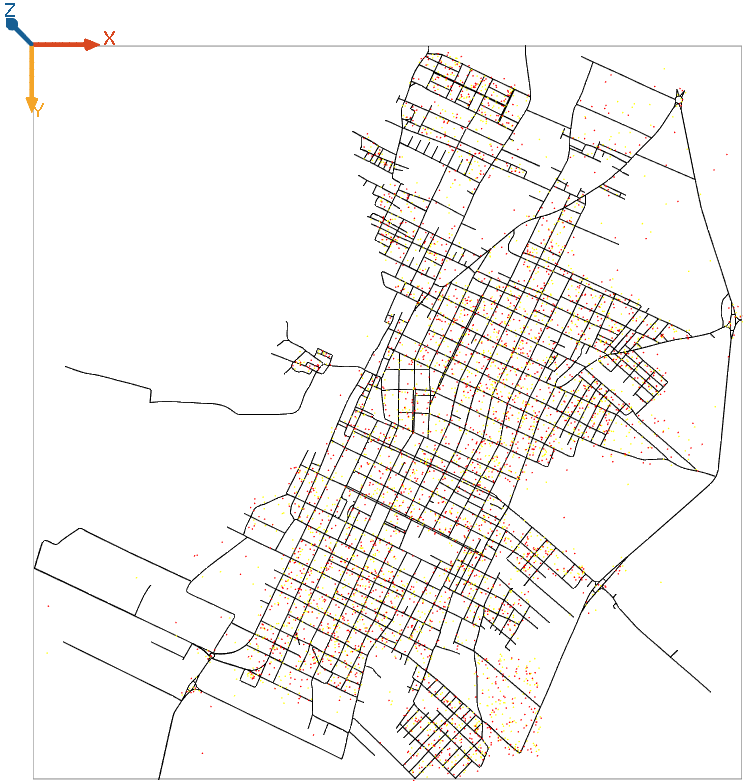
\includegraphics[width=16cm, height=10cm]{images/gama-example.png}
	\caption{Geographic view in GAMA platform.}
	\label{fig:example-gama}
\end{figure}

\section{Data Analysis}\label{sec:data-analysis}

\subsection{Limoeiro do Norte and Alto Santo Cities}\label{subsec:limoeiro-do-norte-and-alto-santo-cities}

This section presents a analysis of the notified cases from the cities of
\textit{Alto Santo} and \textit{Limoeiro do Norte} in the state of Ceará,
Brazil. These notifications are from 2015 to 2022, and they were obtained
through the city health departments through the
\gls{sinan}~\cite{laguardia:2004}. The data is organized in tables that contain
157 information fields from the medical service sheets. From \textit{Alto Santo}
city, we obtained 630 notifications in the data from 2016 to 2022.
\textit{Limoeiro do Norte} city has reported 3829 Dengue and 414 Chikungunya
cases from 2015 to 2021. The data from both cities gives a total of 4873 cases
reported in the \gls{sinan}.

According to the \gls{ibge}\footnote{\url{https://www.ibge.gov.br/}}, in the
last demographic census carried out in 2022, the \textit{Alto Santo} resident
population was 14,155 people. In \textit{Limoeiro}, this value increases to
59,560 residents, more than four times the population of \textit{Alto Santo}.
The urban area of \textit{Alto Santo} is only around 2 km$^2$, while
\textit{Limoeiro} has almost 15 km$^2$. The city centers extracted from the
\gls{osm} are presented in Figure~\ref{fig:osm-graph-examples}.

\begin{figure}[ht!]
	\begin{minipage}[c]{.5\textwidth}
		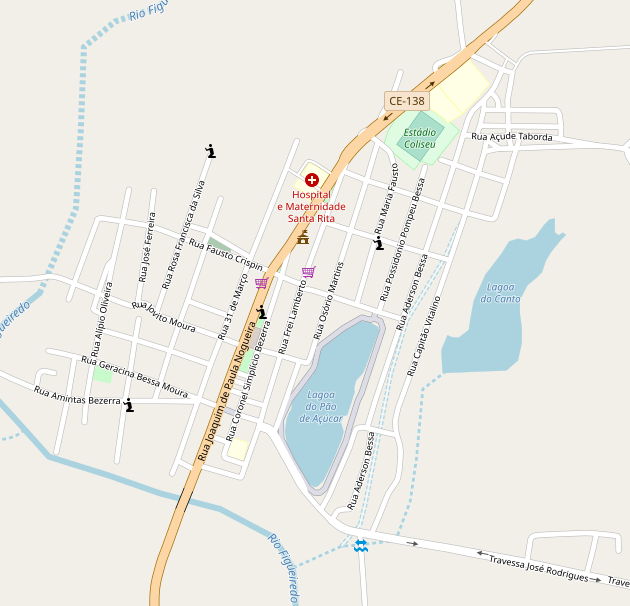
\includegraphics[width=7cm, height=6cm]{images/alto-santo-osm.png}
		\subcaption{Map of Alto Santo downtown.}
	\end{minipage}
	\begin{minipage}[c]{.5\textwidth}
		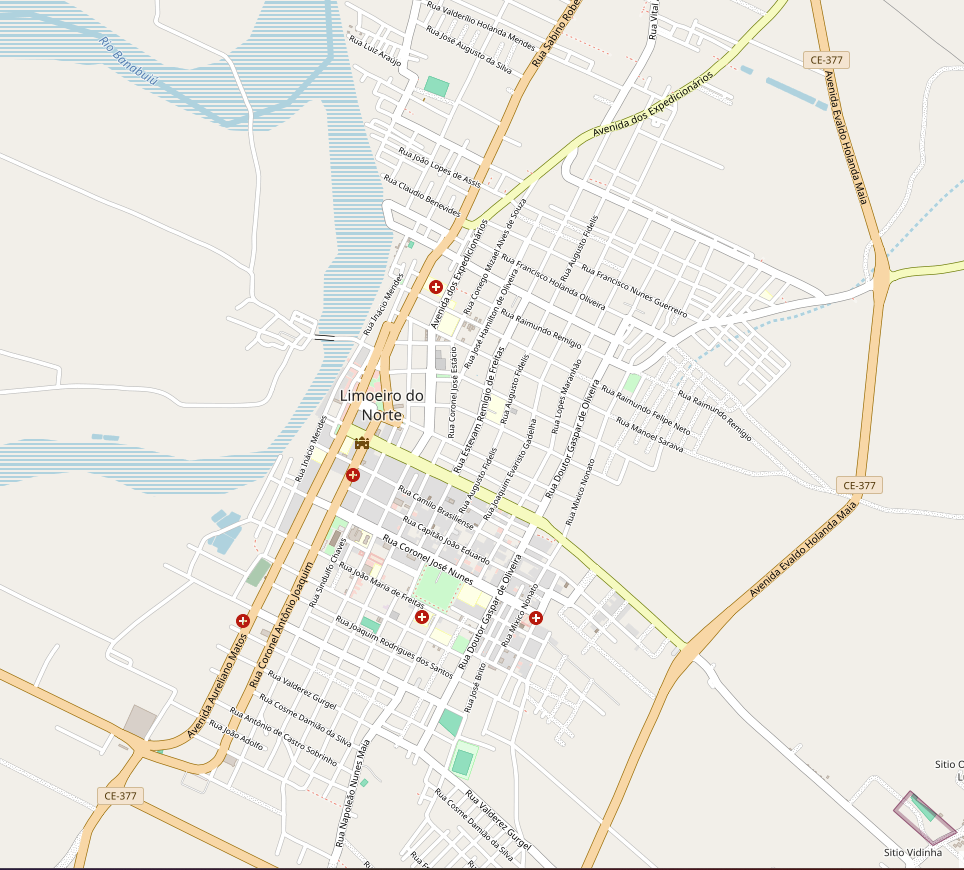
\includegraphics[width=7cm, height=6cm]{images/limoeiro-mapa.png}
		\subcaption{Map of Limoeiro downtown.}
	\end{minipage}
	\caption{\label{fig:osm-graph-examples} Maps extracted from \gls{osm}.}
\end{figure}

Figure~\ref{fig:cases-per-status} shows the number of notifications clustered by
the final classification for the complete \gls{sinan} dataset, including options
such as positive for Dengue or Chikungunya, Dengue with alarm signals, severe
Dengue, discarded cases, and cases pending closure. According to the current
health department of \textit{Alto Santo}, there was underreporting of cases in
the \gls{sinan} during the initial years. This can be observed, for example, in
Figure~\ref{fig:cases-per-year}, which presents the number of notifications
grouped by year for each city. In \textit{Alto Santo}, in 2017, more than 200
notifications remained pending.

\begin{center}
	\begin{figure}[ht!]
		\centering
		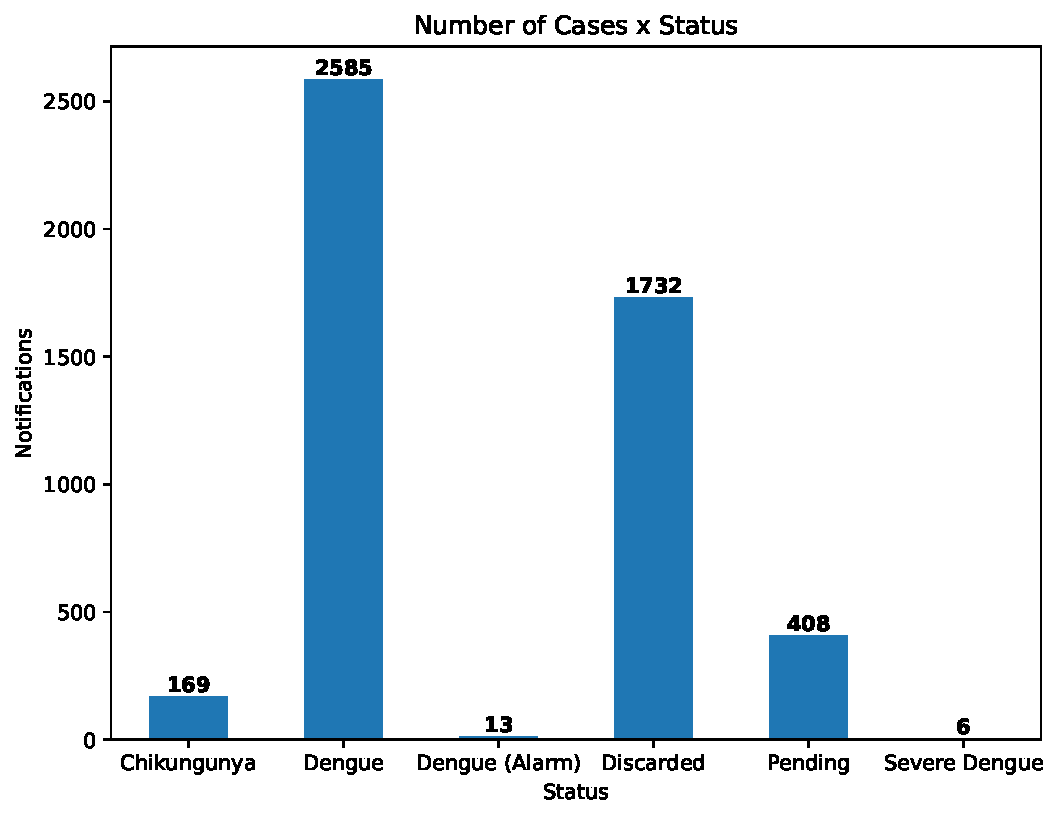
\includegraphics[width=8cm, height=7cm]{images/cases-per-status.pdf}
		\caption{Number of notifications considering both cities under
			study.}\label{fig:cases-per-status}
	\end{figure}
\end{center}

Analyzing the data presented in Figure~\ref{fig:cases-per-year}, except for 2018
in \textit{Limoeiro do Norte}, there are at least 150 positive cases each year,
with the highest number of cases occurring in 2019 and 2020. The year of 2020
was considered an epidemic year, reporting more than 1450 positive cases. In
\textit{Alto Santo}, more than half of the total notifications were reported
only in 2017, with more cases pending than confirmed positive or negative. The
number of positive notifications in all other years is lower than 75 and almost
no cases in the two years after 2017. According to conversations with the
\textit{Alto Santo} health department, except for 2017, none of the years were
characterized as epidemic seasons. The number of cases increased only in 2021.


\begin{center}
	\begin{figure}[ht!]
		\begin{minipage}[c]{.5\textwidth}
			\centering
			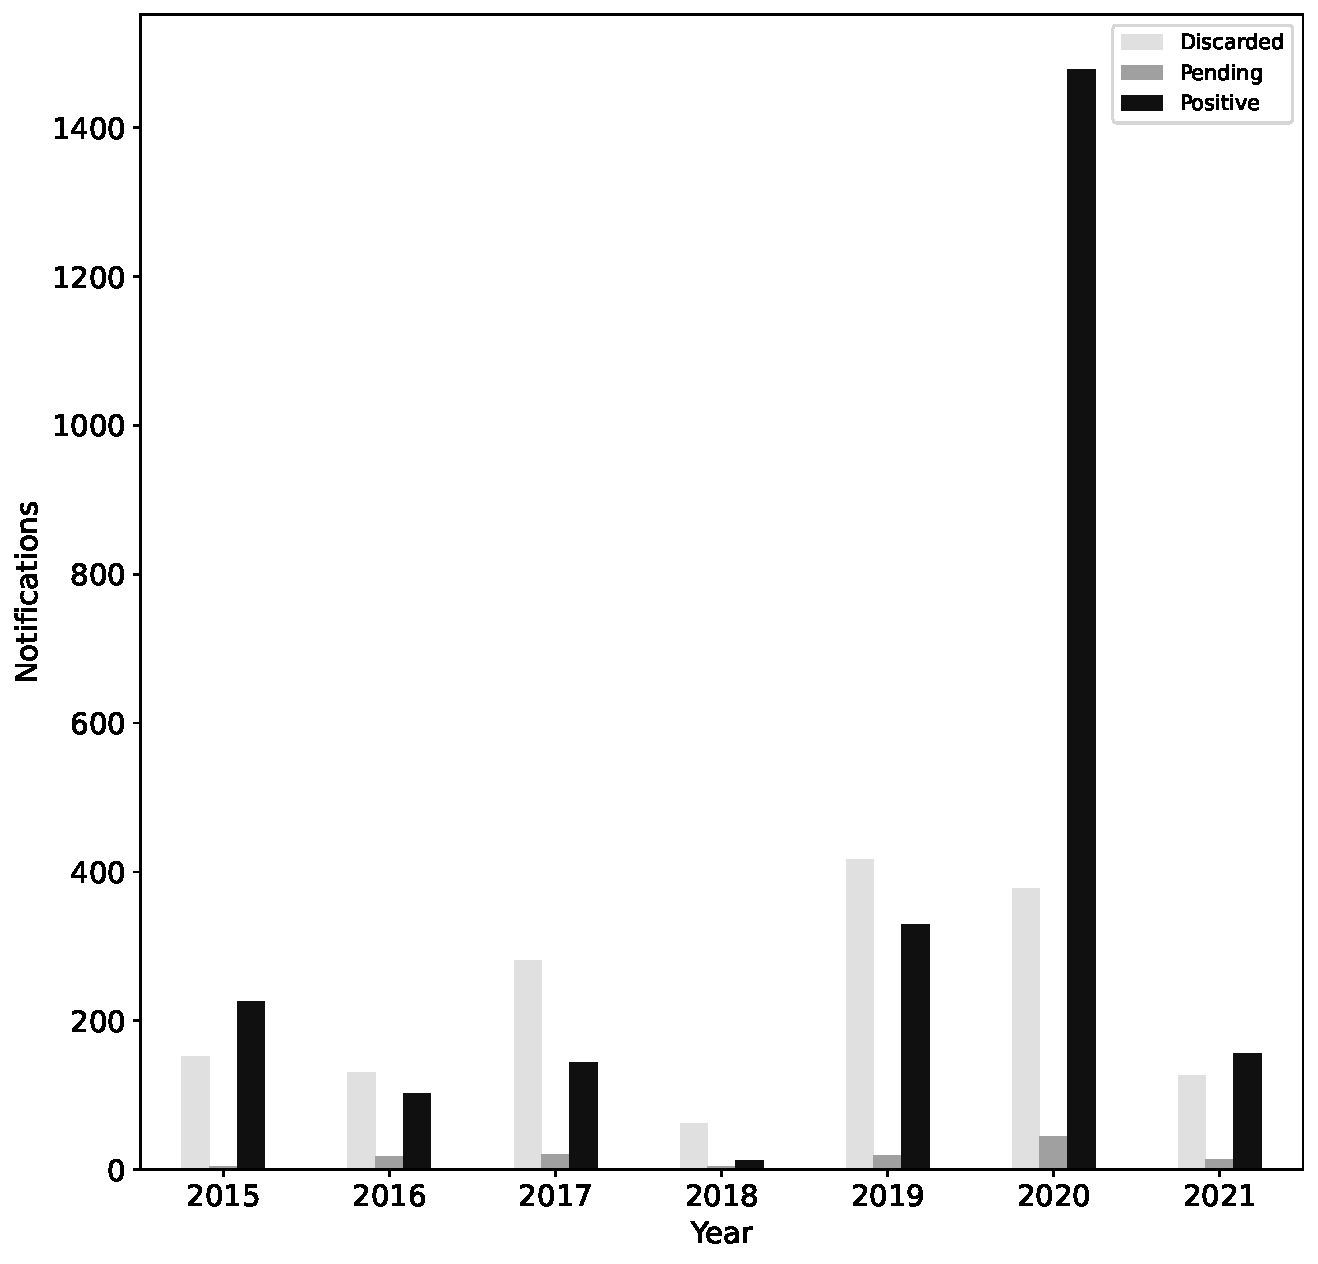
\includegraphics[width=6.5cm, height=7cm]{images/cases-per-year-Limoeiro do Norte.pdf}
			\subcaption{Notifications from Limoeiro.}
		\end{minipage}
		\begin{minipage}[c]{.5\textwidth}
			\centering
			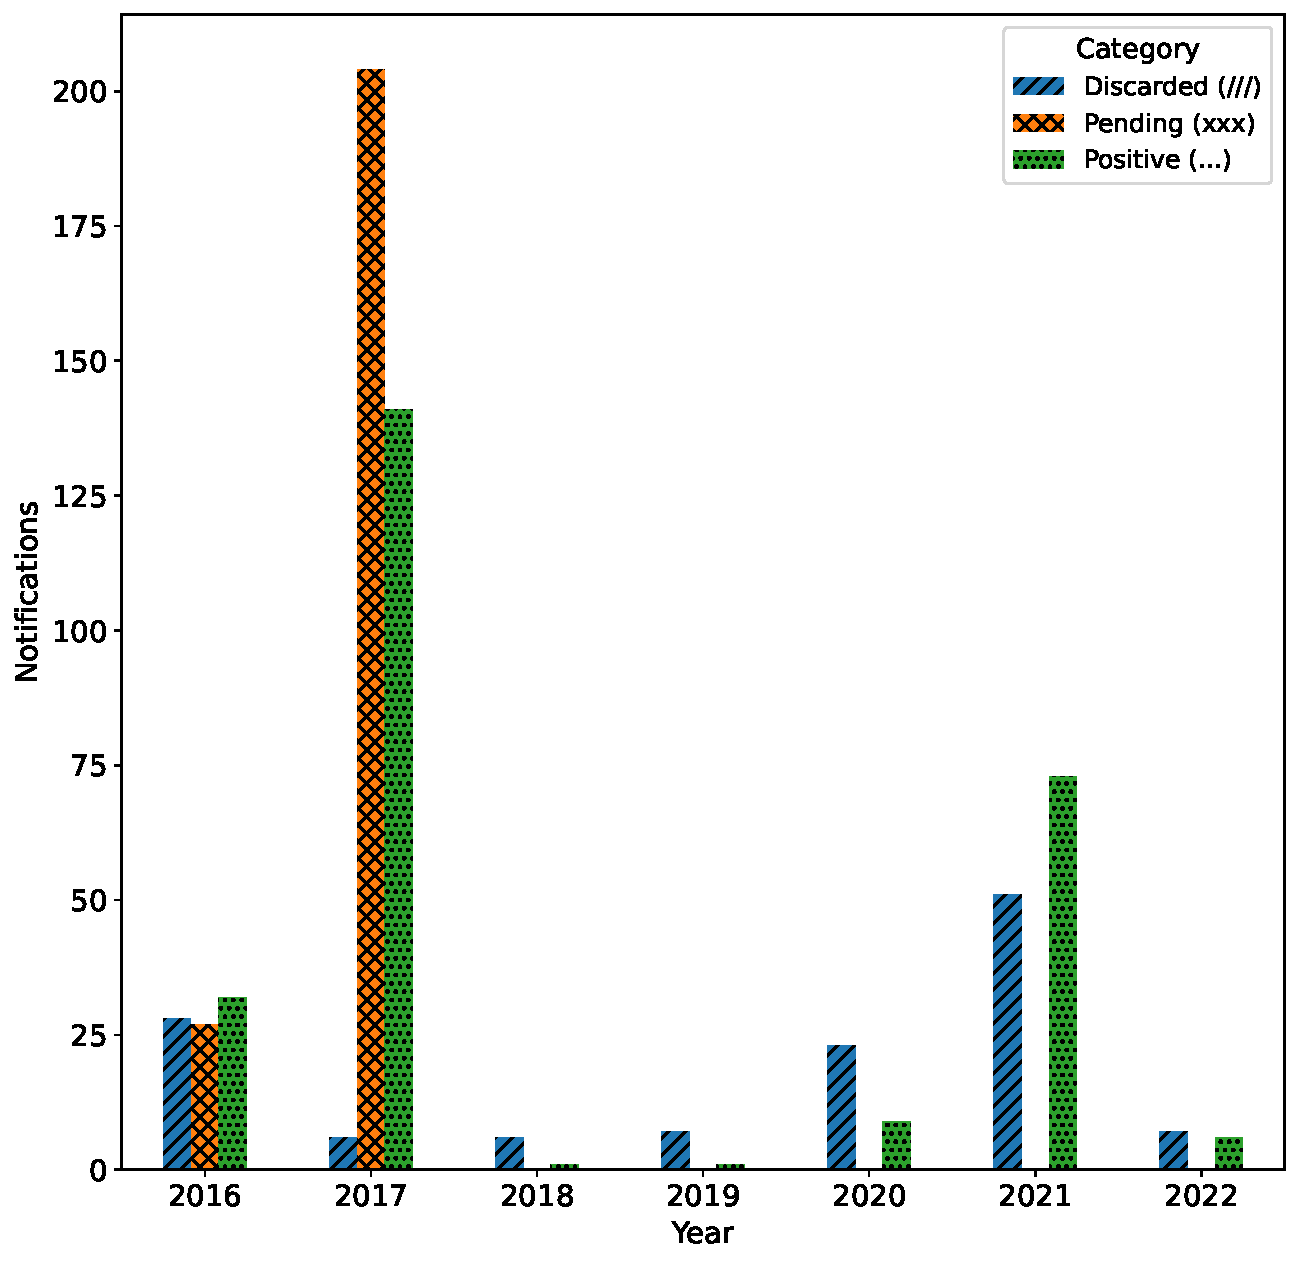
\includegraphics[width=6.5cm, height=7cm]{images/cases-per-year-Alto Santo.pdf}
			\subcaption{Notifications from Alto Santo.}
		\end{minipage}
		\caption{\label{fig:cases-per-year} Number of notifications per year.}
	\end{figure}
\end{center}

Considering the total number of notifications and their distribution over the
years, it is evident that \textit{Limoeiro do Norte}, with a larger population,
also experiences a higher number of Dengue and Chikungunya cases every year. To
analyze the distribution of cases in the same granularity of time used by the
health departments, we selected the two years with the most notifications for
each city, specifically 2019/2020 for \textit{Limoeiro} and 2017/2021 for
\textit{Alto Santo} (Figures~\ref{fig:cases-per-week-limoeiro}
and~\ref{fig:cases-per-week-as}, respectively). These figures depict the
distribution of notifications for each \gls{ew} with at least one notification.

\begin{figure}[ht!]
	\begin{minipage}[c]{.9\textwidth}
		\centering
		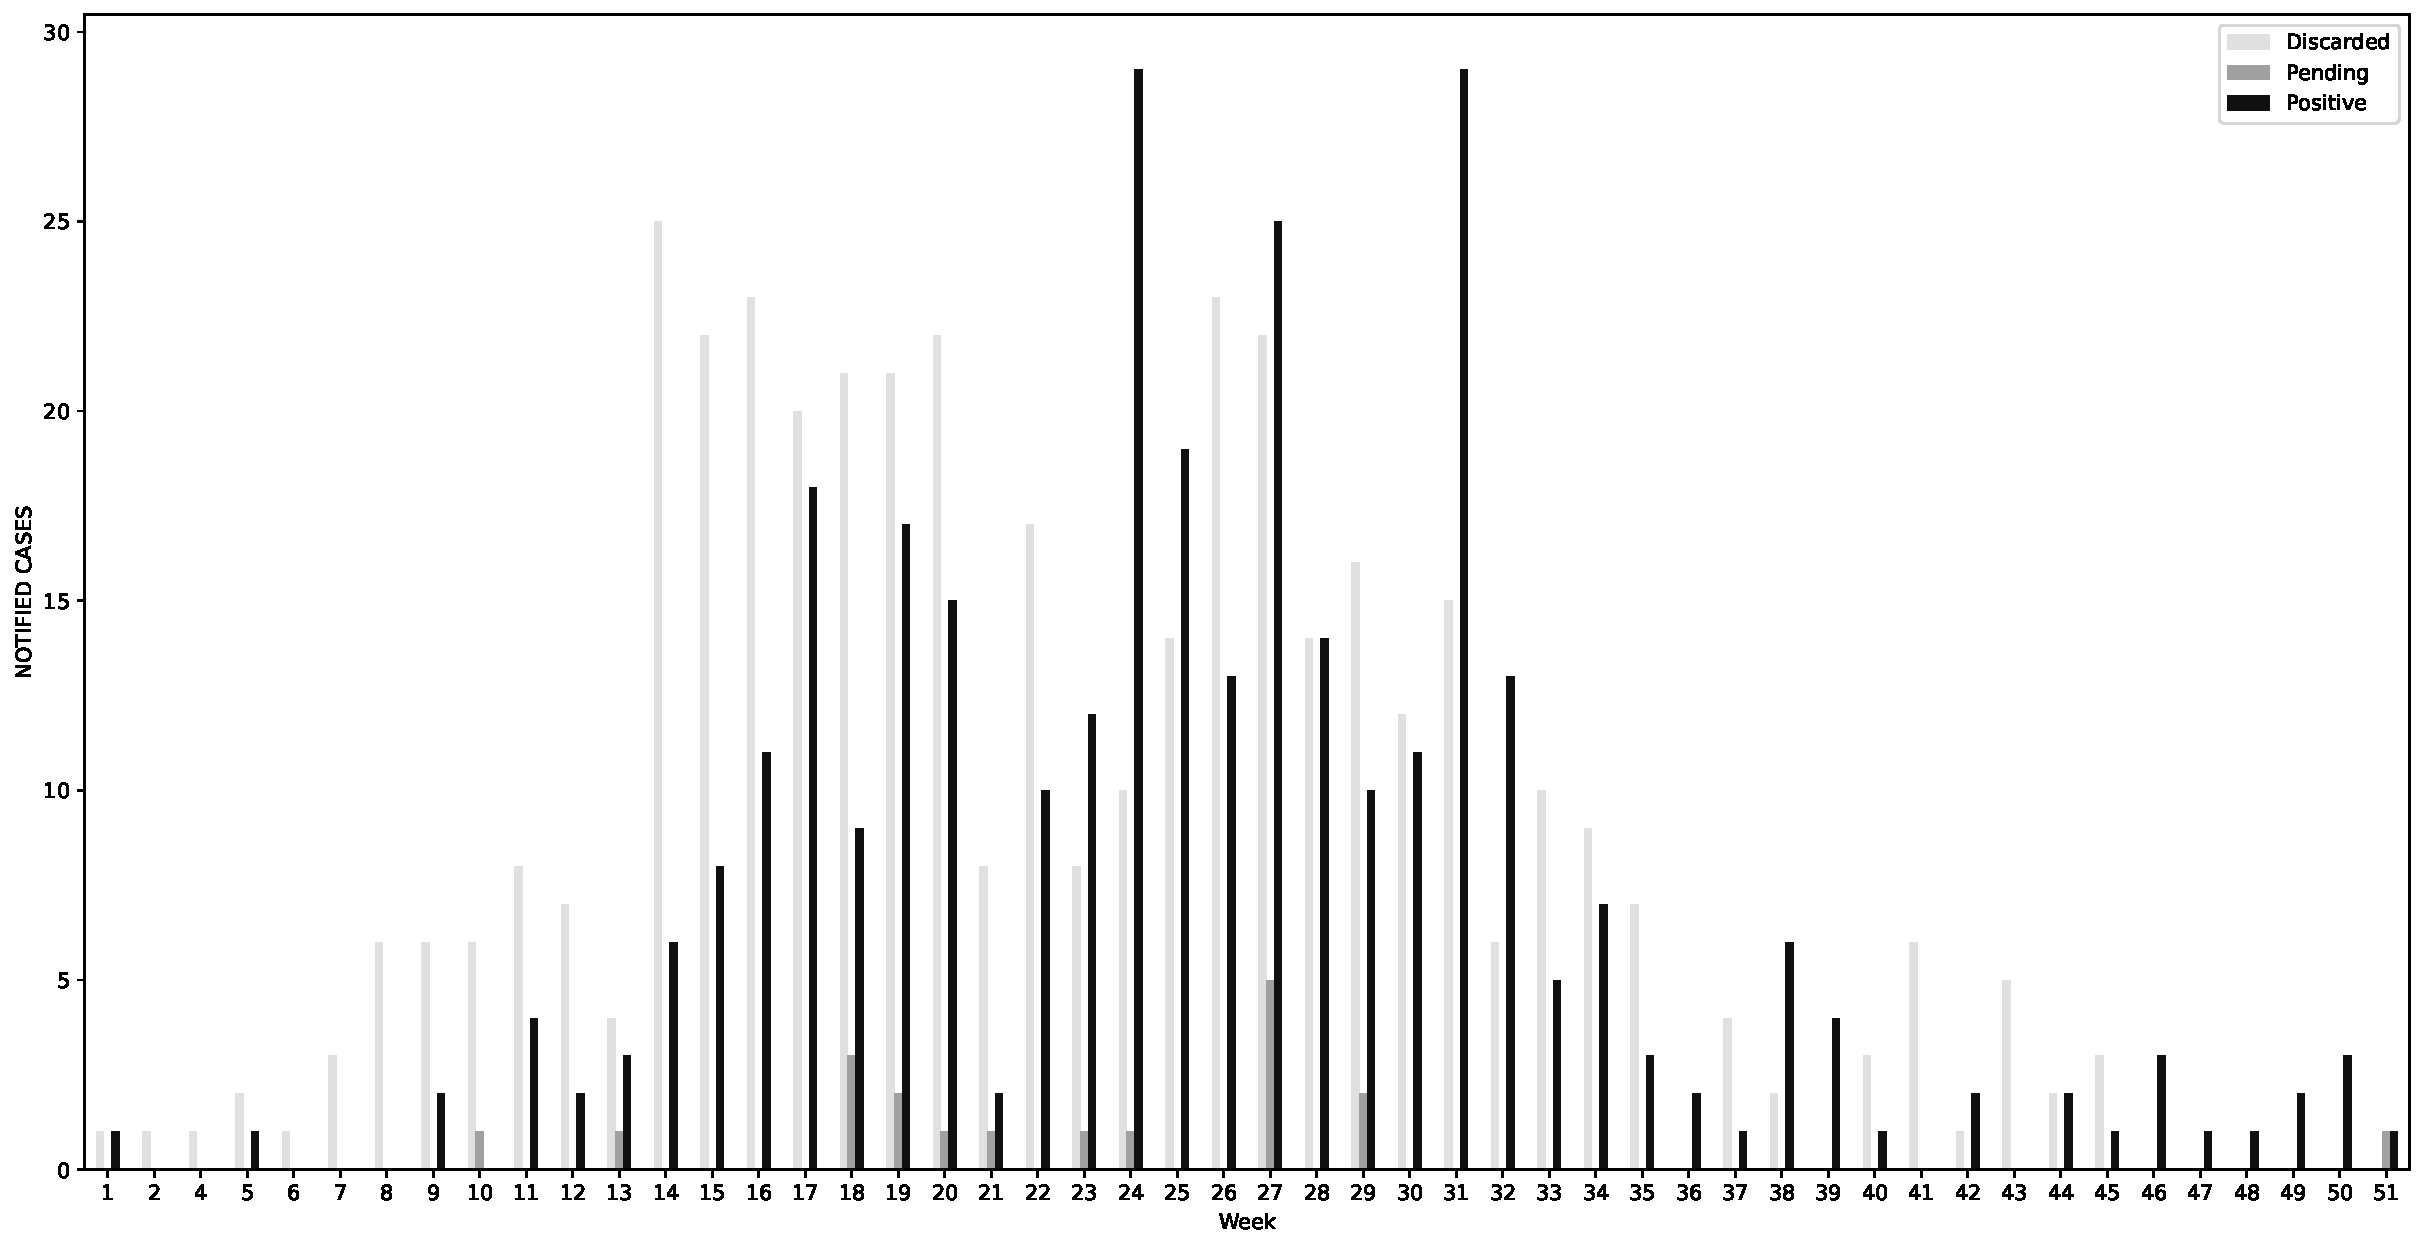
\includegraphics[scale=0.32]{images/cases-per-week-2019-Limoeiro do Norte.pdf}
		\subcaption{Notifications from Limoeiro - 2019.}
	\end{minipage}
	\\
	\begin{minipage}[c]{.9\textwidth}
		\centering
		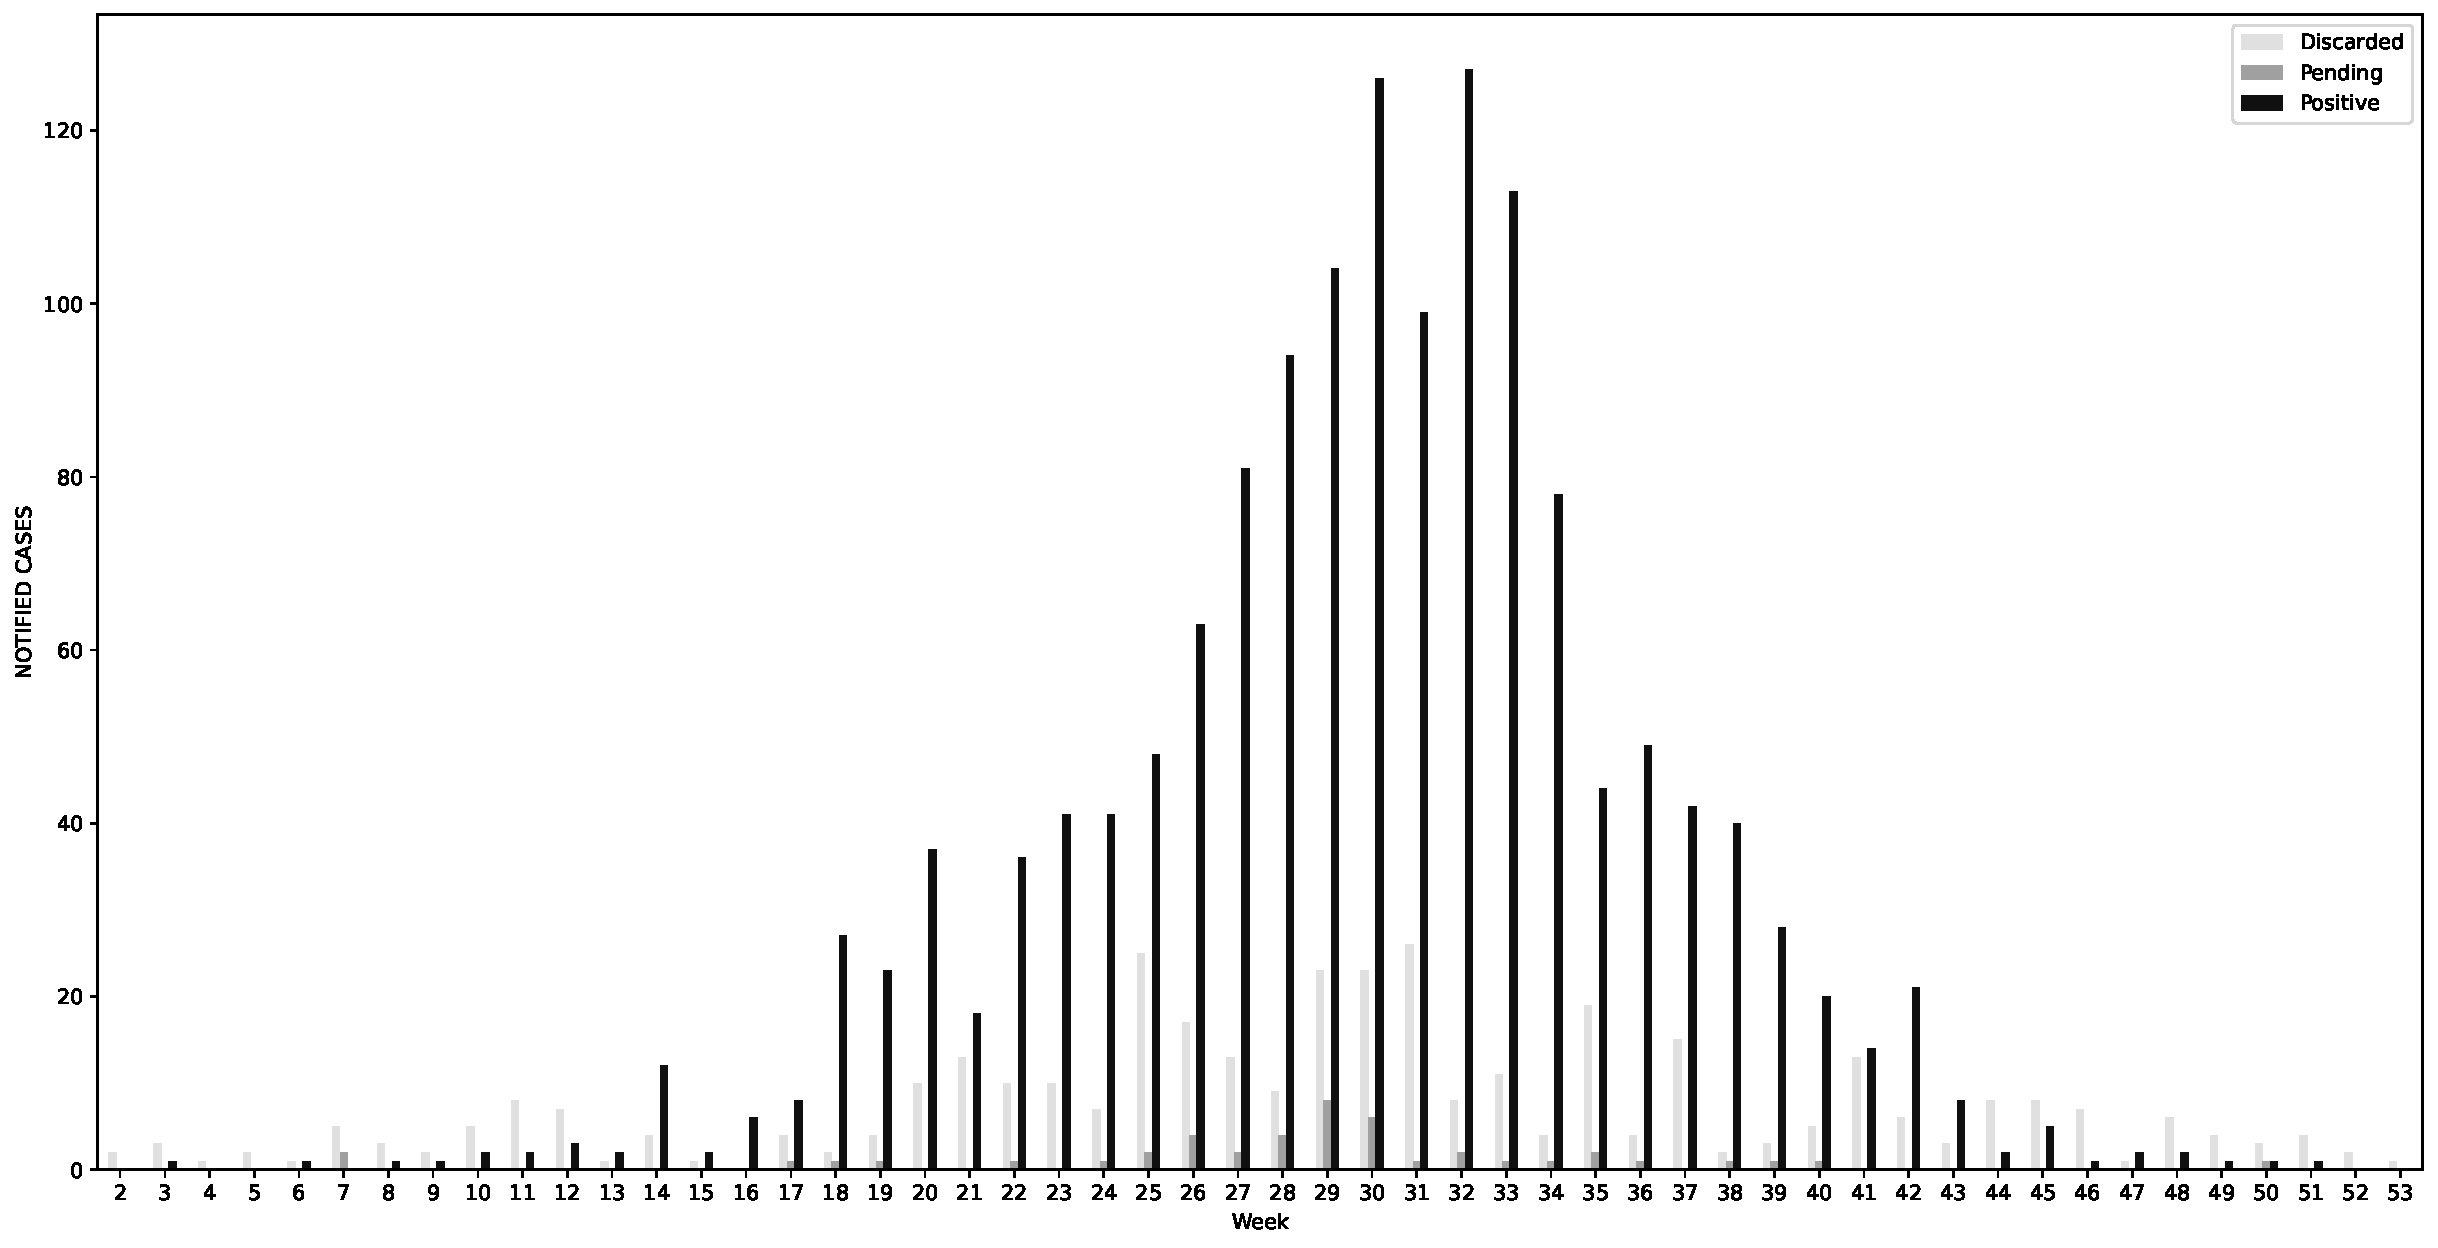
\includegraphics[scale=0.32]{images/cases-per-week-2020-Limoeiro do Norte.pdf}
		\subcaption{Notifications from Limoeiro - 2020.}
	\end{minipage}
	\caption{\label{fig:cases-per-week-limoeiro} Number of notifications per week
		- Limoeiro do Norte.}
\end{figure}

\begin{figure}[ht!]
	\begin{minipage}[c]{.9\textwidth}
		\centering
		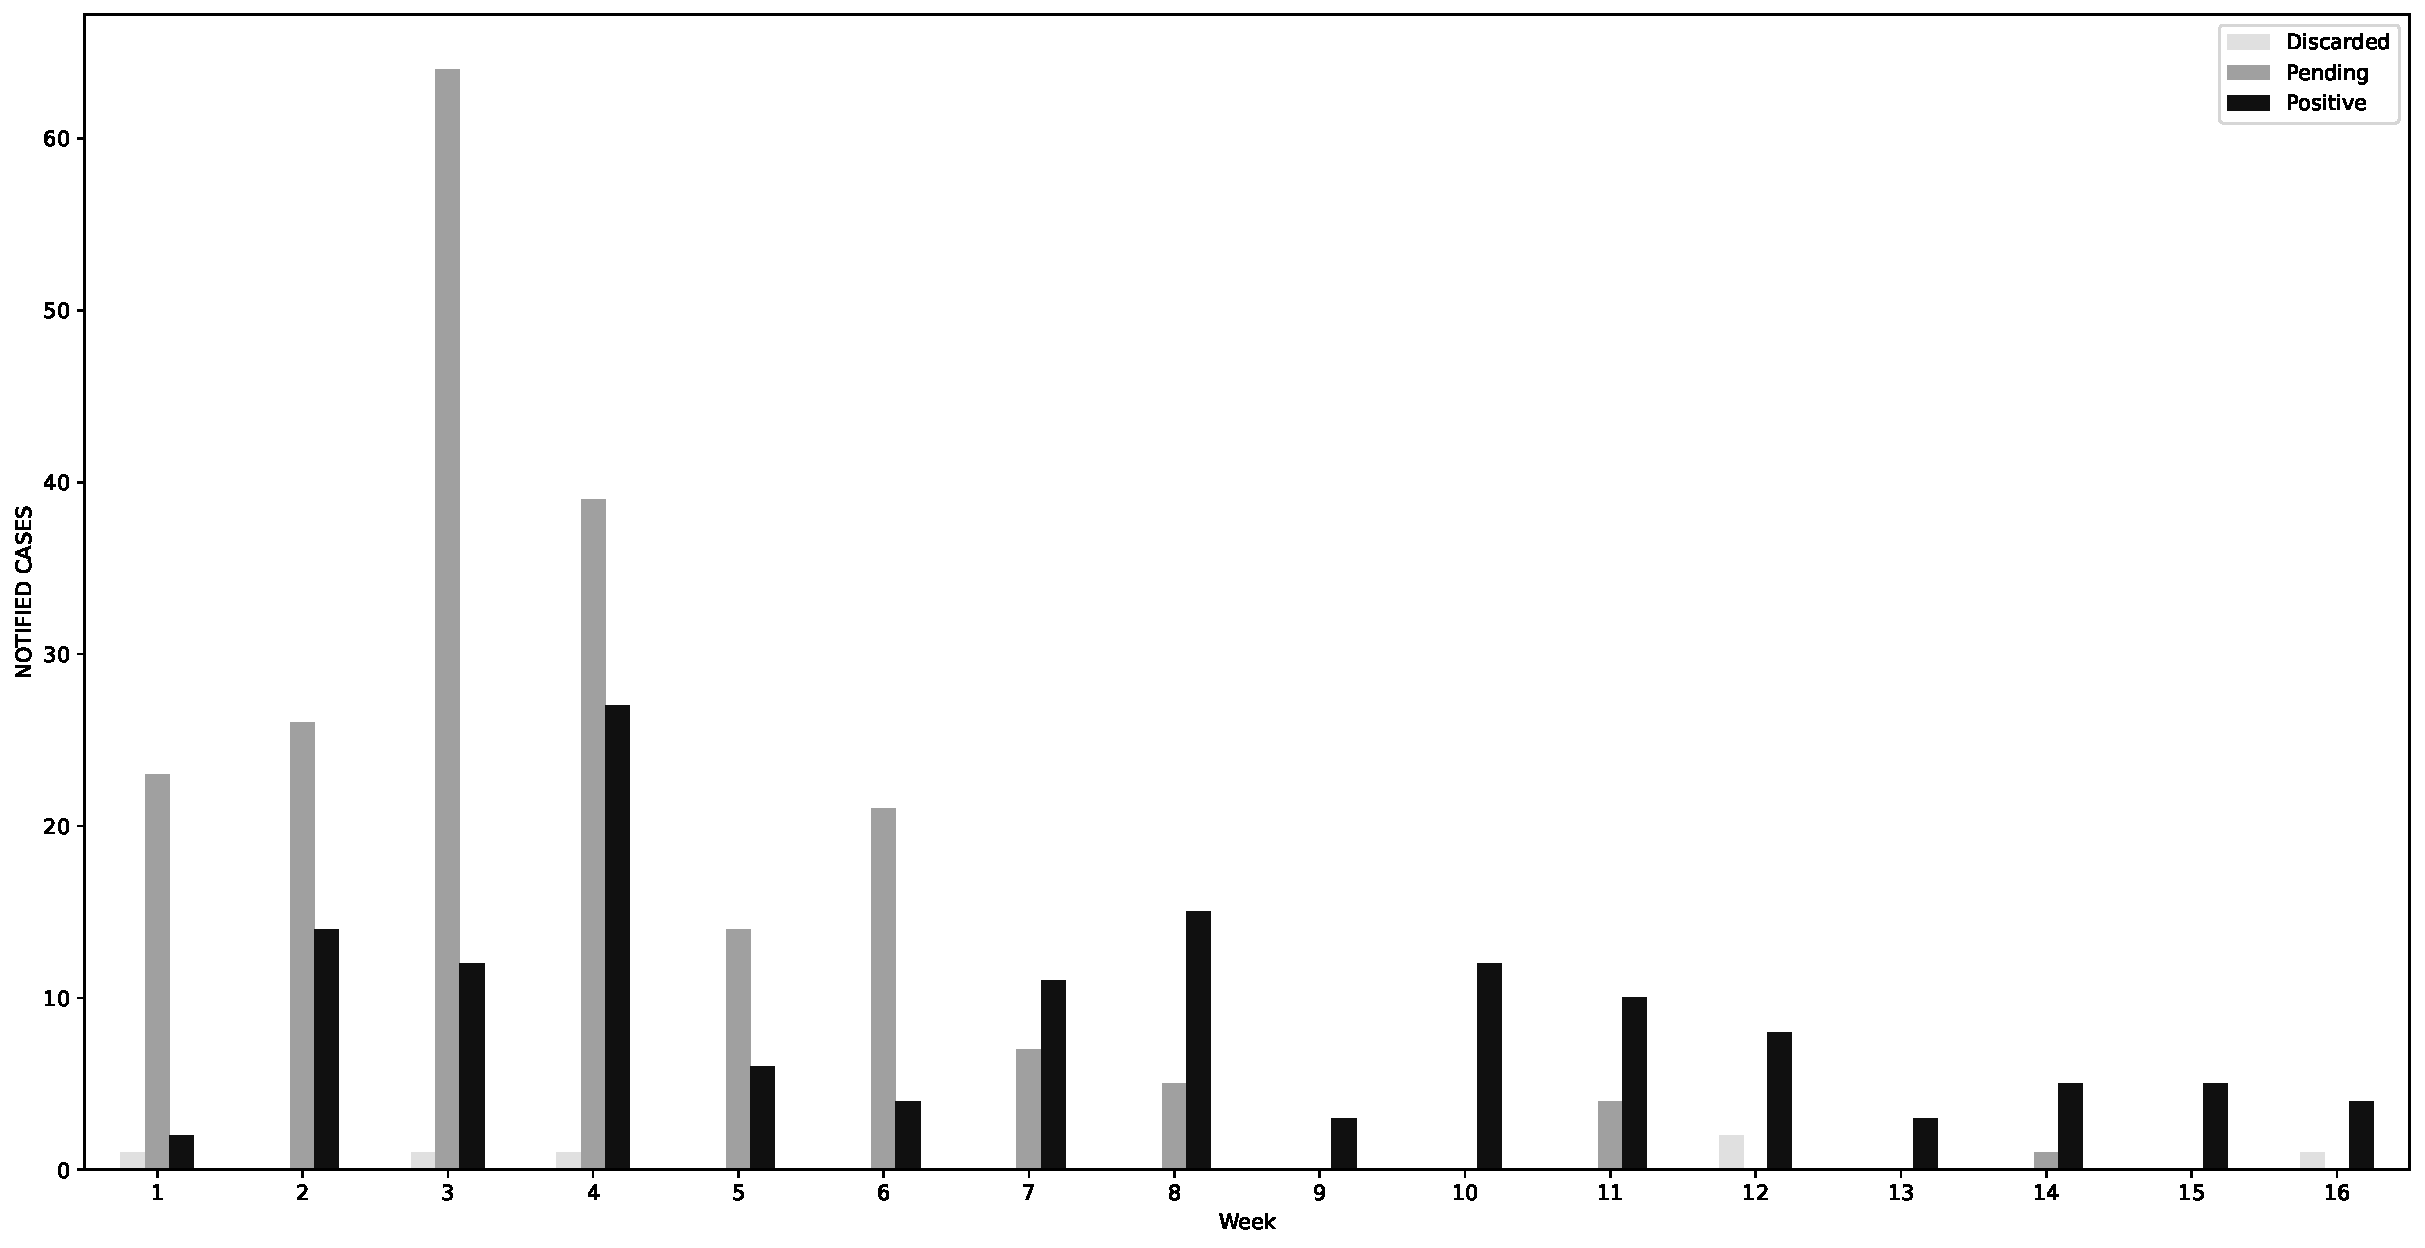
\includegraphics[scale=0.32]{images/cases-per-week-2017-Alto Santo.pdf}
		\subcaption{Notifications from Alto Santo - 2017.}
	\end{minipage}
	\\
	\begin{minipage}[c]{.9\textwidth}
		\centering
		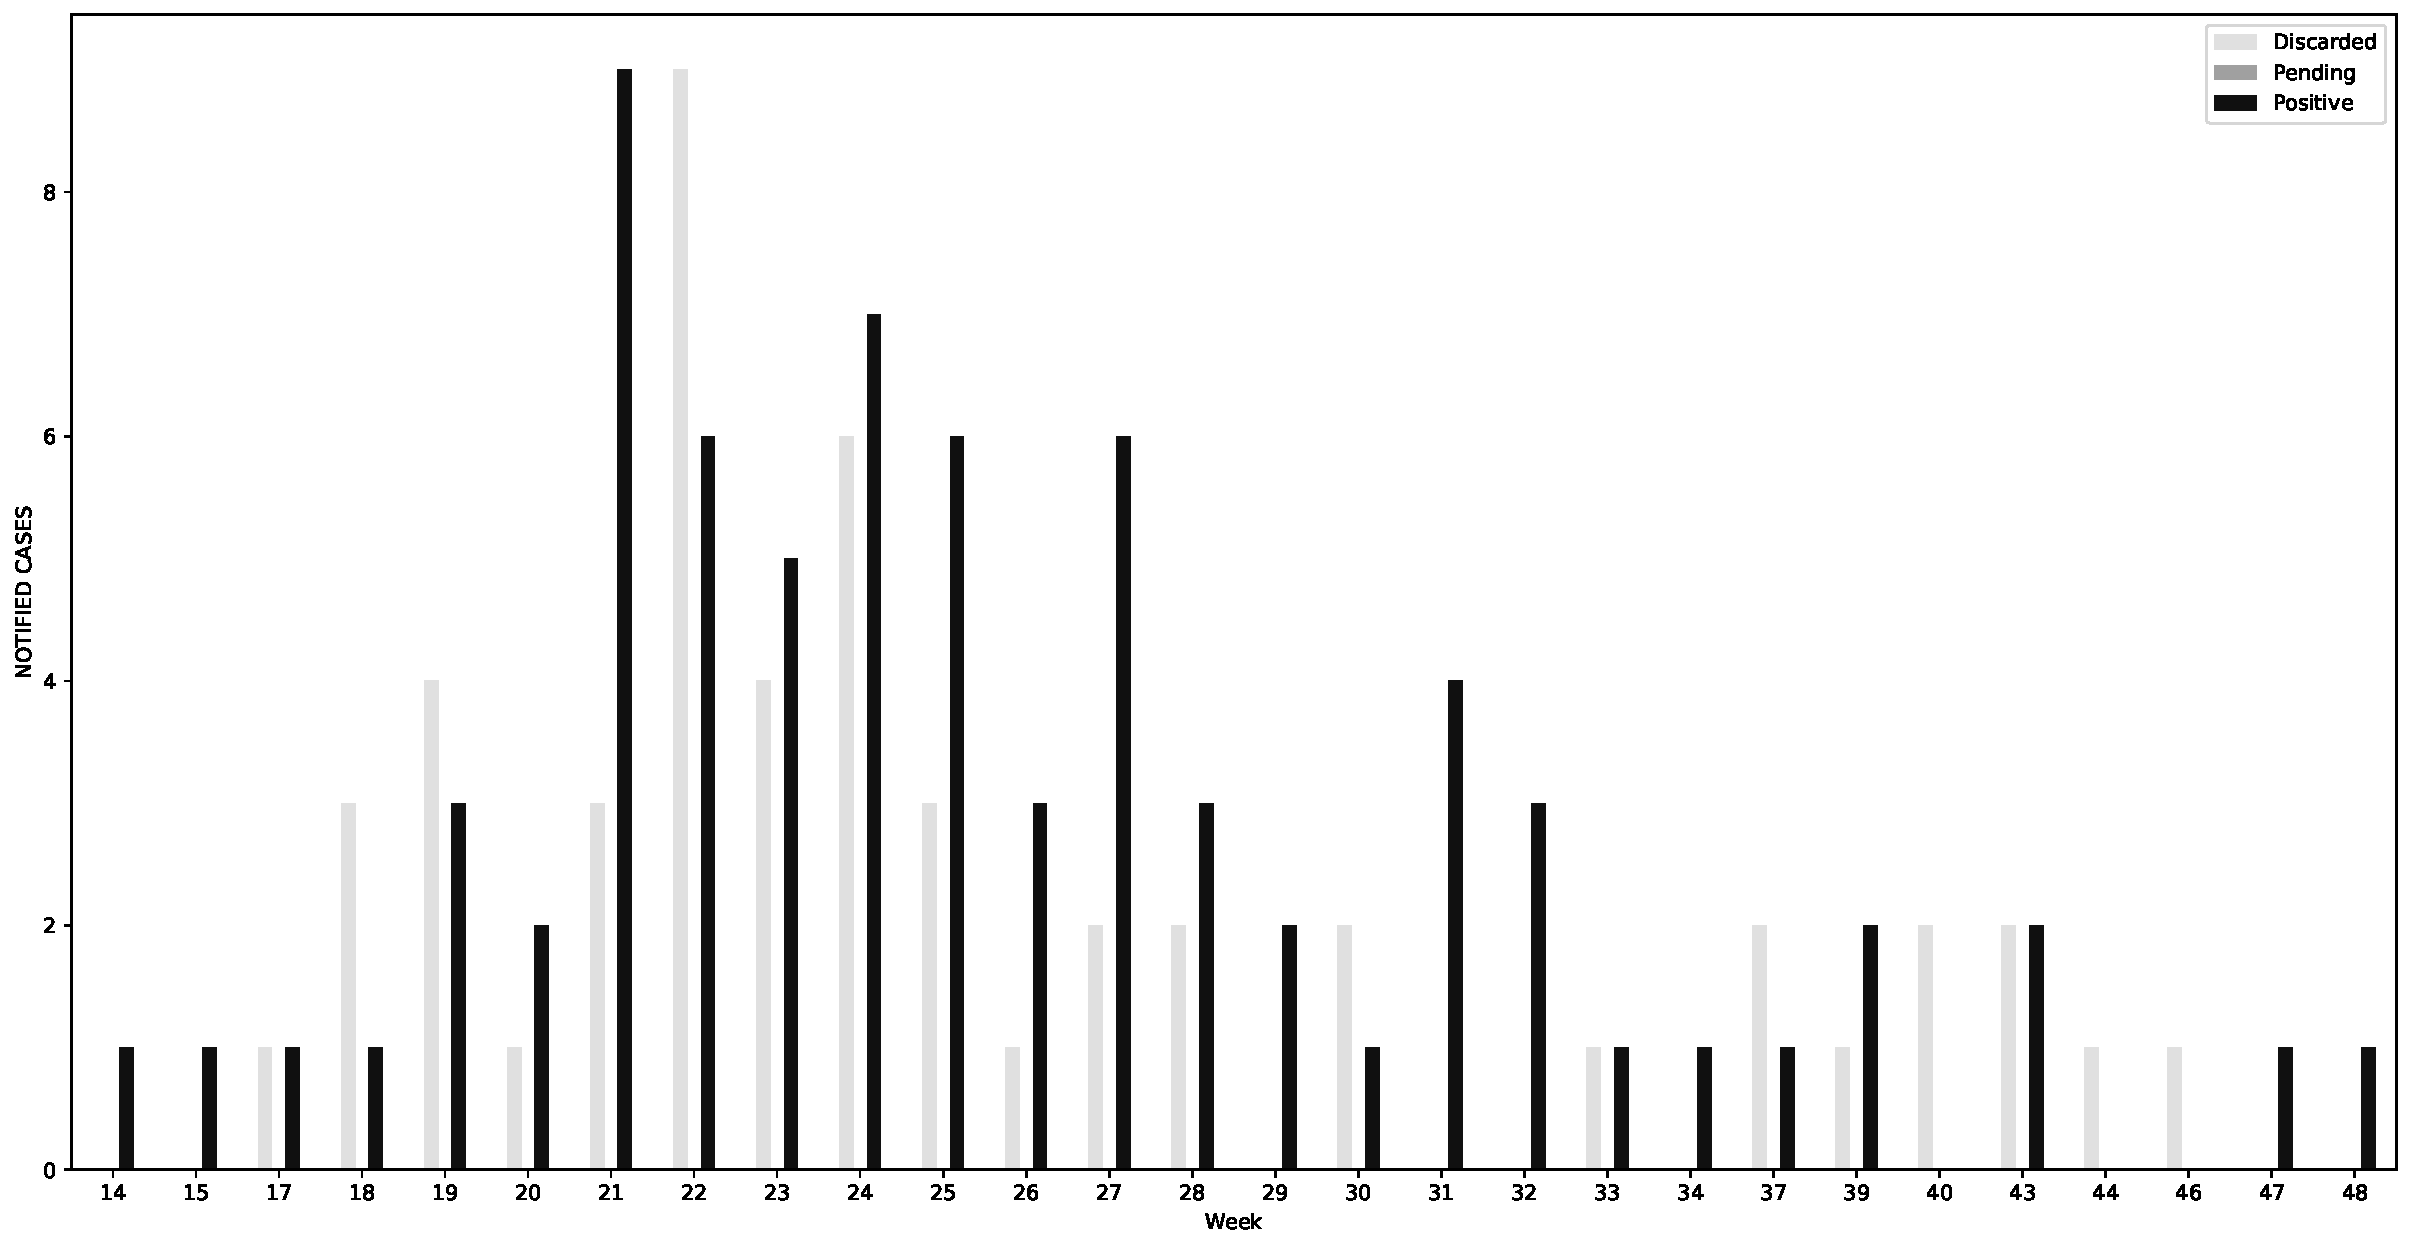
\includegraphics[scale=0.32]{images/cases-per-week-2021-Alto Santo.pdf}
		\subcaption{Notifications from Alto Santo - 2021.}
	\end{minipage}
	\caption{\label{fig:cases-per-week-as} Number of notifications per week - Alto
		Santo.}
\end{figure}


In \textit{Alto Santo}, during 2017, dengue cases were reported within the first
16 epidemiological weeks (\gls{ews}), peaking at 25 cases in week 4. Based on
the application, we can classify these notifications as either positive or
negative, given the high number of confirmed dengue cases during the same
period. In 2021, cases were recorded between \gls{ew} 14 and 48, with a lower
weekly incidence, reaching a peak of 9 confirmed cases in week 21.

From \textit{Limoeiro}, in 2019, cases are present in almost all weeks with
peaks of positive cases occurring between weeks 24 and 32, ranging from 10 to 29
cases. There is an epidemic season from weeks 20 to 38 of 2020, where the number
of cases is at least 40, and for 8 consecutive weeks after the 27 \gls{ew}, the
number of cases ranges from 80 to 123.

Two points need to be highlighted to understand this dataset. First,
underreporting likely occurred as infected individuals may not have pursued
hospital care due to: \textit{(1)} Knowing Dengue is seasonal, individuals often
self-diagnose when experiencing common disease symptoms, \textit{(2)} adherence
to clinically recommended protocols without formal testing, or \textit{(3)} mild
symptoms that did not disrupt daily activities. Second, the absence of
spatiotemporal records on vector-control interventions (e.g., insecticide
campaigns and larval habitat removal) obscures their impact on mosquito
populations and localized transmission dynamics. These limitations collectively
contribute to the observed fluctuations in notifications.

In both cities, public health strategies lack integration with digital
surveillance tools or predictive systems. Unfortunately, they rely on reactive
containment measures initiated only after spikes in confirmed dengue cases. This
firefighting approach - common across resource-constrained municipalities in
Brazil - fails to optimize prevention due to three key gaps: \textit{(i)}
delayed detection of epidemiological trends, \textit{(ii)} absence of
data-driven risk mapping to prioritize high-risk zones, and \textit{(iii)} ad
hoc resource allocation that overlooks transmission dynamics. Consequently,
interventions often occur too late to curb outbreaks effectively, perpetuating
cycles of suboptimal public health outcomes.

\section{Statistical Analysis of Results}\label{subsec:statistical-analysis}

\section{Instance Generation}\label{sec:instance-generation}

To identify (label) each city block, we employ a graph-theoretical procedure
that corresponds to finding the faces of a planar
embedding~\citep{diestel2024graph}. A planar embedding, also called a rotation
system, is defined for a planar graph by assigning, for each vertex $( i \in V
	)$, a cyclic ordering $C(i)$ of its neighbors (typically in clockwise order).
Intuitively, this defines the clockwise order of streets around each
intersection. This rotation system can be computed using the geometric slope of
each incident arc~\citep{PhilipKleinShayMozes}. As an illustrative example,
consider the graph in \ref{fig:non_isolated_nodes}. Its planar embedding can be
described by the function $C$ as shown in Table~\ref{tabnew}.

\begin{figure}[ht!]
	\centering
	\begin{tikzpicture}[>=latex]
		% nodes
		% block A
		\coordinate (A1) at (0.1, 2.9);
		\coordinate (A2) at (1.9, 2.9);
		\coordinate (A3) at (1.9, 2);
		\coordinate (A4) at (1.9, 1.1);
		\coordinate (A5) at (0.1, 1.1);
		\coordinate (BorderA1) at (0, 3);
		\coordinate (BorderA2) at (2, 3);
		\coordinate (BorderA3) at (2, 2);
		\coordinate (BorderA4) at (2, 1);
		\coordinate (BorderA5) at (0, 1);
		% block B
		\coordinate (B1) at (2.1, 2.9);
		\coordinate (B2) at (3.9, 2.9);
		\coordinate (B3) at (3.9, 1.1);
		\coordinate (B4) at (2.1, 1.1);
		\coordinate (B5) at (2.1, 2);
		\coordinate (BorderB1) at (2, 3);
		\coordinate (BorderB2) at (4, 3);
		\coordinate (BorderB3) at (4, 1);
		\coordinate (BorderB4) at (2, 1);
		\coordinate (BorderB5) at (2, 2);
		% block C
		\coordinate (C1) at (2, 0.9);
		\coordinate (C2) at (2.9, 0.1);
		\coordinate (C3) at (1.1, 0.1);
		\coordinate (BorderC1) at (2, 1);
		\coordinate (BorderC2) at (3.1, 0);
		\coordinate (BorderC3) at (0.9, 0);
		% block B
		\coordinate (D1) at (2, 3.1);
		\coordinate (D2) at (1.1, 3.9);
		\coordinate (D3) at (2.9, 3.9);
		\coordinate (BorderD1) at (2, 3);
		\coordinate (BorderD2) at (0.9, 4);
		\coordinate (BorderD3) at (3.1, 4);
		% blocks
		\def\blockA{A1, A2, A3, A4, A5}
		\def\blockB{B1, B2, B3, B4, B5}
		\def\blockC{C1, C2, C3}
		\def\blockD{D1, D2, D3}
		% arcs
		\def\arcs{%
			% block A
			BorderA1 BorderA2
			BorderA2 BorderA3
			BorderA3 BorderA4
			BorderA4 BorderA5
			BorderA5 BorderA1
			% block B
			BorderB1 BorderB2
			BorderB2 BorderB3
			BorderB3 BorderB4
			BorderB4 BorderB5
			BorderB5 BorderB1
			% block C
			BorderC1 BorderC2
			BorderC2 BorderC3
			BorderC3 BorderC1
			% block D
			BorderD1 BorderD2
			BorderD2 BorderD3
			BorderD3 BorderD1
		}
		\readarray\arcs\Arcs[16,2]
		% print arcs
		\drawArcs{\Arcs}{\ArcsROWS}{->, gray!20, to path={-| (\tikztotarget)}}
		%block A
		\drawBlock{A1}{\blockA}{red!50};
		%block B
		\drawBlock{B1}{\blockB}{black!50};
		%block C
		\drawBlock{C1}{\blockC}{yellow!50};
		%block D
		\drawBlock{D1}{\blockD}{blue!50};
		% dot
		\filldraw[black] (BorderD1) circle (1pt);
		% blocks labels
		% A
		\node[xshift=2mm, yshift=-1.5mm] at (0.8, 2.2) {$b_1$};
		\node[xshift=2mm, yshift=-1.5mm] at (A1) {\tiny$b_1^1$};
		\node[xshift=-2mm, yshift=-1.5mm] at (A2) {\tiny$b_1^2$};
		\node[xshift=-2mm, yshift=1.5mm] at (A3) {\tiny$b_1^3$};
		\node[xshift=-2mm, yshift=1.5mm] at (A4) {\tiny$b_1^4$};
		\node[xshift=2mm, yshift=1.5mm] at (A5) {\tiny$b_1^5$};
		% B
		\node[xshift=2mm, yshift=-1.5mm] at (2.8, 2.2) {$b_2$};
		\node[xshift=2mm, yshift=-1.5mm] at (B1) {\tiny$b_2^1$};
		\node[xshift=-2mm, yshift=-1.5mm] at (B2) {\tiny$b_2^2$};
		\node[xshift=-2mm, yshift=1.5mm] at (B3) {\tiny$b_2^3$};
		\node[xshift=2mm, yshift=1.5mm] at (B4) {\tiny$b_2^4$};
		\node[xshift=2mm, yshift=1.5mm] at (B5) {\tiny$b_2^5$};
		% C
		\node[xshift=2mm, yshift=-1.5mm] at (1.8, 0.5) {$b_3$};
		\node[yshift=-1.5mm] at (C1) {\tiny$b_3^1$};
		\node[xshift=-4mm, yshift=1.5mm] at (C2) {\tiny$b_3^2$};
		\node[xshift=4mm, yshift=1.5mm] at (C3) {\tiny$b_3^3$};
		% B
		\node[xshift=2mm, yshift=-1.5mm] at (1.8, 3.85) {$b_4$};
		\node[yshift=2.5mm] at (D1) {\tiny$b_4^1$};
		\node[xshift=4.5mm, yshift=-1.5mm] at (D2) {\tiny$b_4^2$};
		\node[xshift=-4.5mm, yshift=-1.5mm] at (D3) {\tiny$b_4^3$};
	\end{tikzpicture}
	\caption{Example of non-isolated street-blocks.}
	\label{fig:non_isolated_nodes}
\end{figure}


\begin{table}[h!]
	\centering
	\caption{Connections for each city block}\label{tabnew}
	\begin{tabular}{cl}
		\hline
		\textbf{City Block} & \textbf{Connections}                      \\ \hline
		\( C(b^1_1) \)      & \( (b^5_1, b^2_1) \)                      \\
		\( C(b^2_1) \)      & \( (b^3_1, b^1_1, b^2_4, b^3_4, b^2_2) \) \\
		\( C(b^3_1) \)      & \( (b^4_1, b^1_2) \)                      \\
		\( C(b^4_1) \)      & \( (b^3_3, b^5_1, b^5_2, b^3_2, b^2_3) \) \\
		\( C(b^5_1) \)      & \( (b^1_1, b^4_1) \)                      \\
		\( C(b^2_2) \)      & \( (b^1_2, b^3_2) \)                      \\
		\( C(b^3_2) \)      & \( (b^4_2, b^2_2) \)                      \\
		\( C(b^2_3) \)      & \( (b^3_3, b^1_3) \)                      \\
		\( C(b^3_3) \)      & \( (b^1_3, b^2_3) \)                      \\
		\( C(b^2_4) \)      & \( (b^3_4, b^1_4) \)                      \\
		\( C(b^3_4) \)      & \( (b^1_4, b^2_4) \)                      \\ \hline
	\end{tabular}
\end{table}

With combinatorial embedding \( C \) and arc set \( A \), we identify all
bounded and unbounded faces of the planar graph using a traversal procedure
formalized in Algorithm~\ref{alg:find_faces}. Each face corresponds to a cyclic
sequence of arcs that form the boundary of a region enclosed by streets (i.e., a
city block). The algorithm iteratively traverses unused arcs in the graph by
following the clockwise ordering defined by \( C \), marking each arc as visited
once it has been assigned to a face. Each traversal terminates upon returning to
the starting arc, thus completing a cycle (face). This procedure ensures that
every face is uniquely defined by a sequence of arcs traversed in the clockwise
direction relative to the embedding. We note that every planar embedding has one
unbounded `outer' face encircling the whole graph. This outer face does not
correspond to any physical city block, so we exclude it from the set of labeled
blocks.


\begin{algorithm}[h!]
	\caption{Face-finding algorithm for planar embedding}
	\label{alg:find_faces}
	\begin{algorithmic}[1]
		\REQUIRE Planar graph \( D = (V, A) \), combinatorial embedding \( C \)
		\ENSURE Set of directed cycles \( \mathcal{F} \) representing faces

		\STATE Initialize \( \mathcal{F} \gets \emptyset \), and mark all arcs in \( A \) as unvisited
		\FOR{each unvisited arc \( a = (u, v) \in A \)}
		\STATE Set \( a_0 \gets a \), and mark \( a \) as visited
		\REPEAT
		\STATE Append \( a \) to \( f \)
		\STATE Let \( w \) be the next vertex after \( u \) in \( C(v) \) (i.e., clockwise successor of \( u \))
		\STATE Set \( a \gets (v, w) \); mark \( a \) as visited
		\STATE Update \( u \gets v \), \( v \gets w \)
		\UNTIL{\( a = a_0 \)}
		\STATE Add \( f \) to \( \mathcal{F} \)
		\ENDFOR
		\RETURN \( \mathcal{F} \)
	\end{algorithmic}
\end{algorithm}

\subsection{Real-case instances}\label{subsec:real_instances}

We collected real-world dengue notification data from 2015 to 2021 through the
municipal health departments of Alto Santo and Limoeiro do Norte, located in the
state of Ceará, Brazil. The data were extracted from the
\gls{sinan}~\cite{laguardia:2004}. During this period, Alto Santo reported 582
cases (2016-2021), and Limoeiro do Norte reported 4,243 cases (2015-2021),
totaling 4,825 confirmed dengue cases between the two cities. Our computational
benchmark consists of 39 instances based on these notifications. The addresses
of reported cases were geolocated using the OSMnx library~\cite{boeing:2017},
which provided latitude and longitude coordinates. Each case was mapped to its
corresponding city block, allowing us to integrate the case data with the street
network. Figure~\ref{fig:graph-examples} illustrates both the geographic maps and the
corresponding graph models of Alto Santo and Limoeiro do Norte, as derived from \gls{osm}. Figure~\ref{tab:real-instances} summarizes the key characteristics
of the benchmark used in the experimental evaluation.

\begin{figure}[h!]
	\begin{minipage}[c]{.49\textwidth}
		\centering
		\subfloat[Map of Alto Santo from OSM.]{\label{fig:altosanto}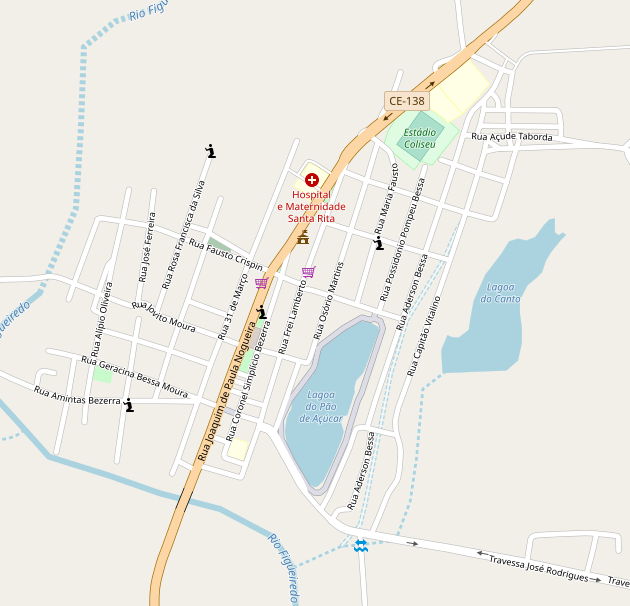
\includegraphics[width=7cm, height=6cm]{images/alto-santo-osm.png}}
	\end{minipage}%
	\begin{minipage}[c]{.49\textwidth}
		\centering
		\subfloat[Map of Limoeiro do Norte from OSM.]{\label{fig:limoeiro}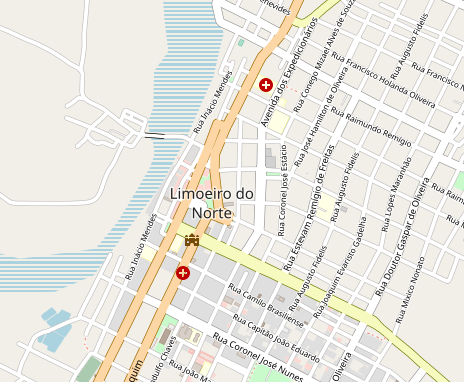
\includegraphics[width=7cm, height=6cm]{images/limoeiro-osm.png}}
	\end{minipage}\\[2mm]
	\begin{minipage}[c]{.49\textwidth}
		\centering
		\subfloat[Graph of Alto Santo.]{\label{fig:Galtosanto}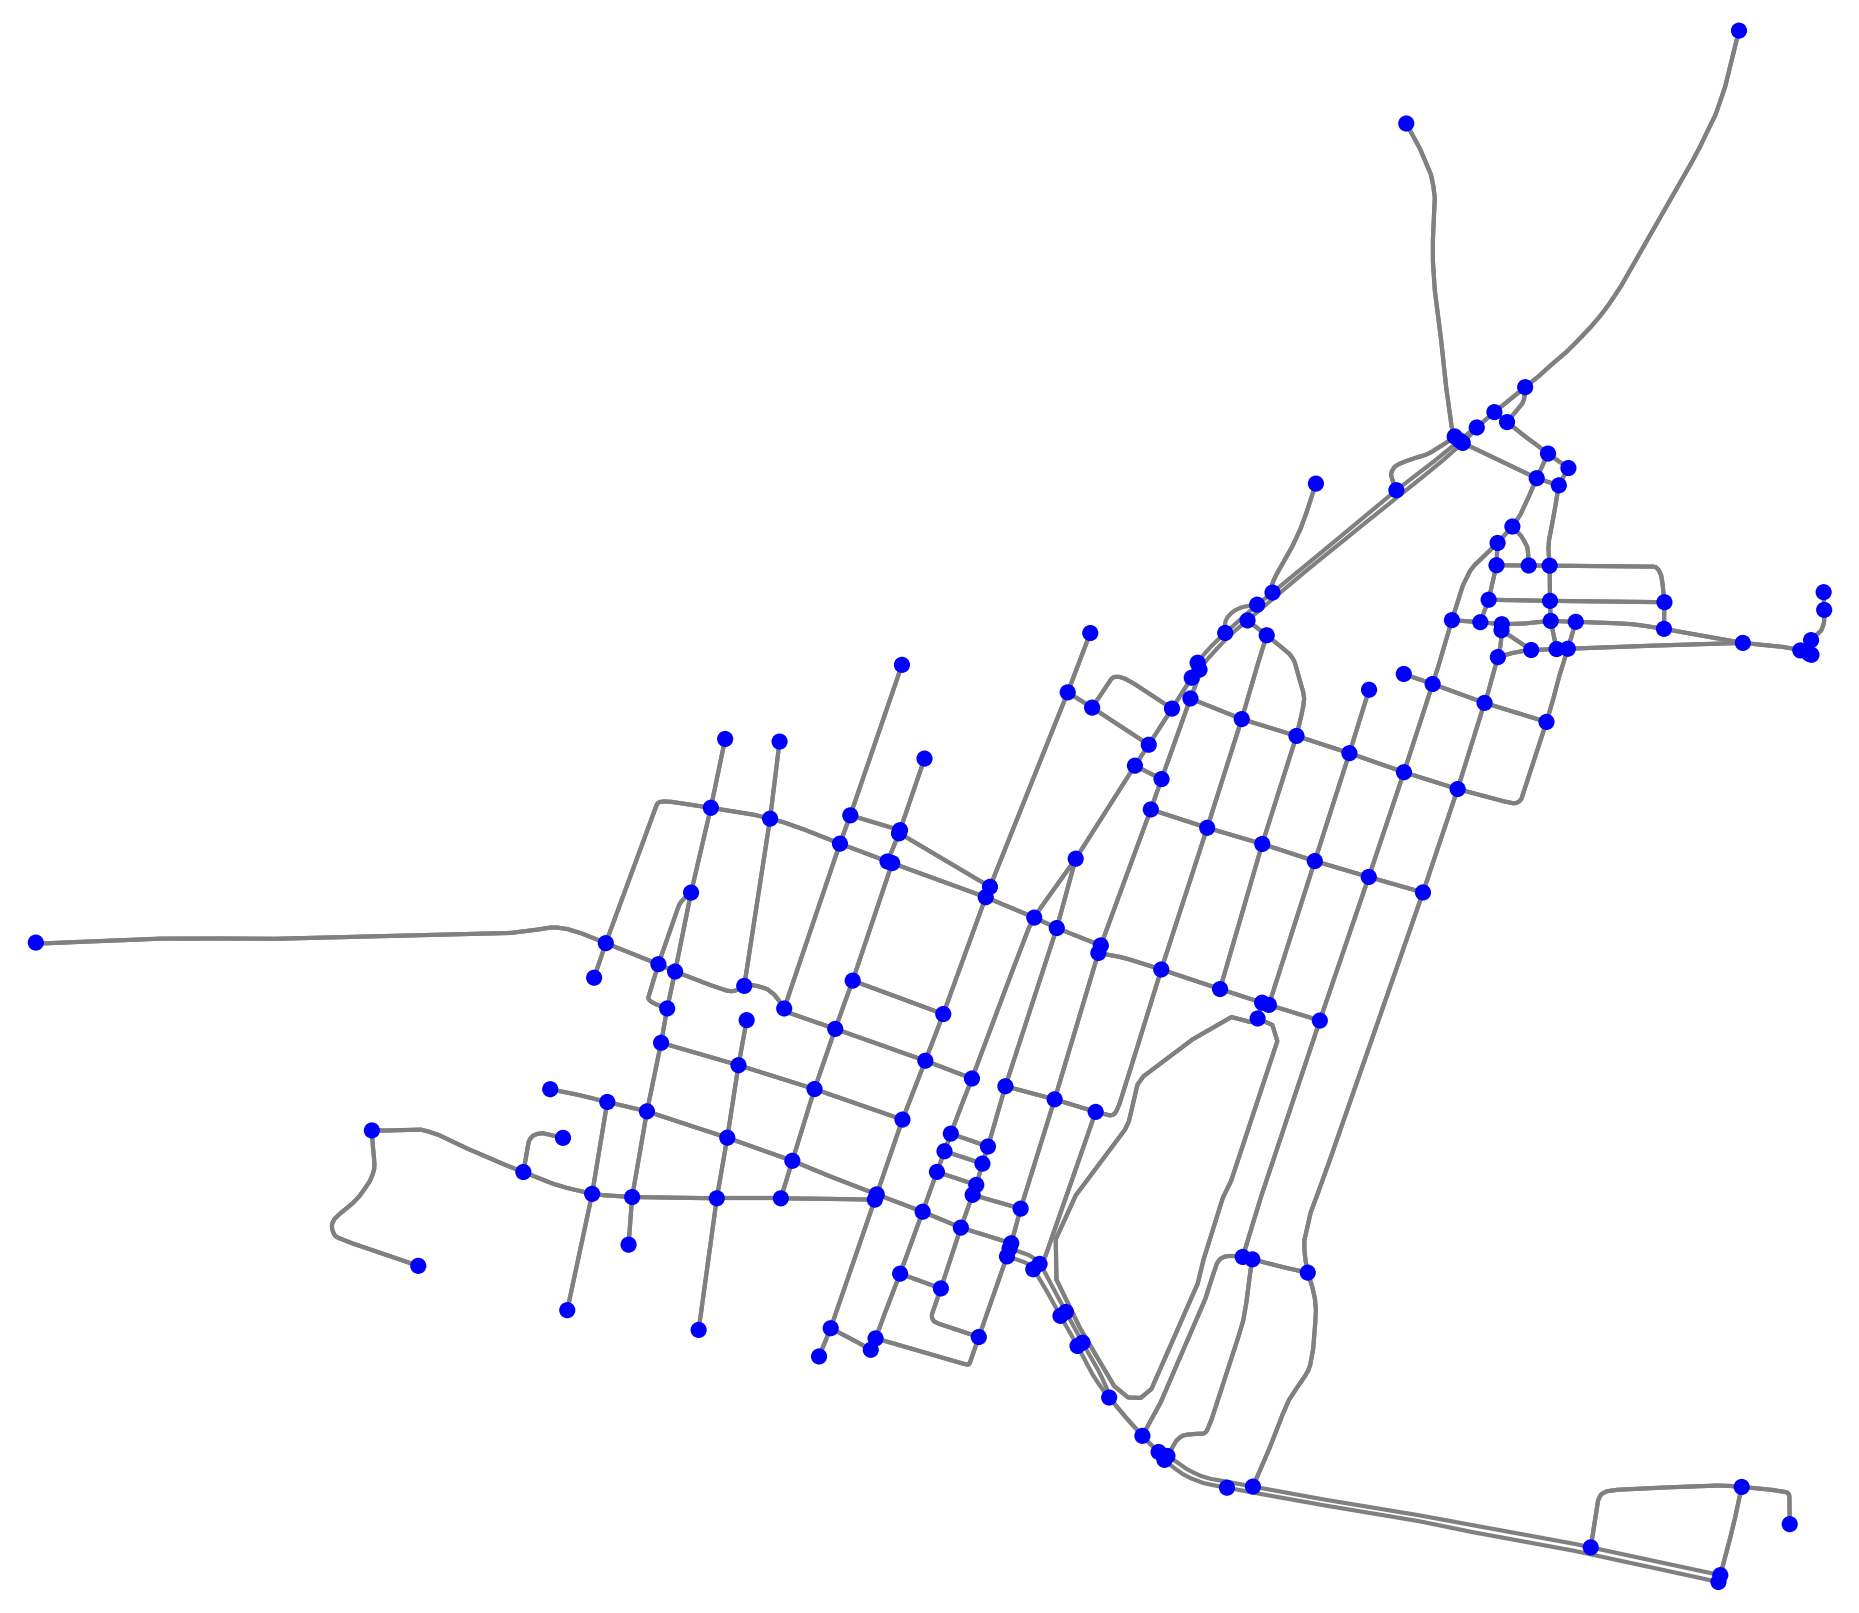
\includegraphics[width=7cm, height=6cm]{images/graph-alto-santo.png}}
	\end{minipage}%
	\begin{minipage}[c]{.49\textwidth}
		\centering
		\subfloat[Graph of Limoeiro do Norte.]{\label{fig:Glimoeiro}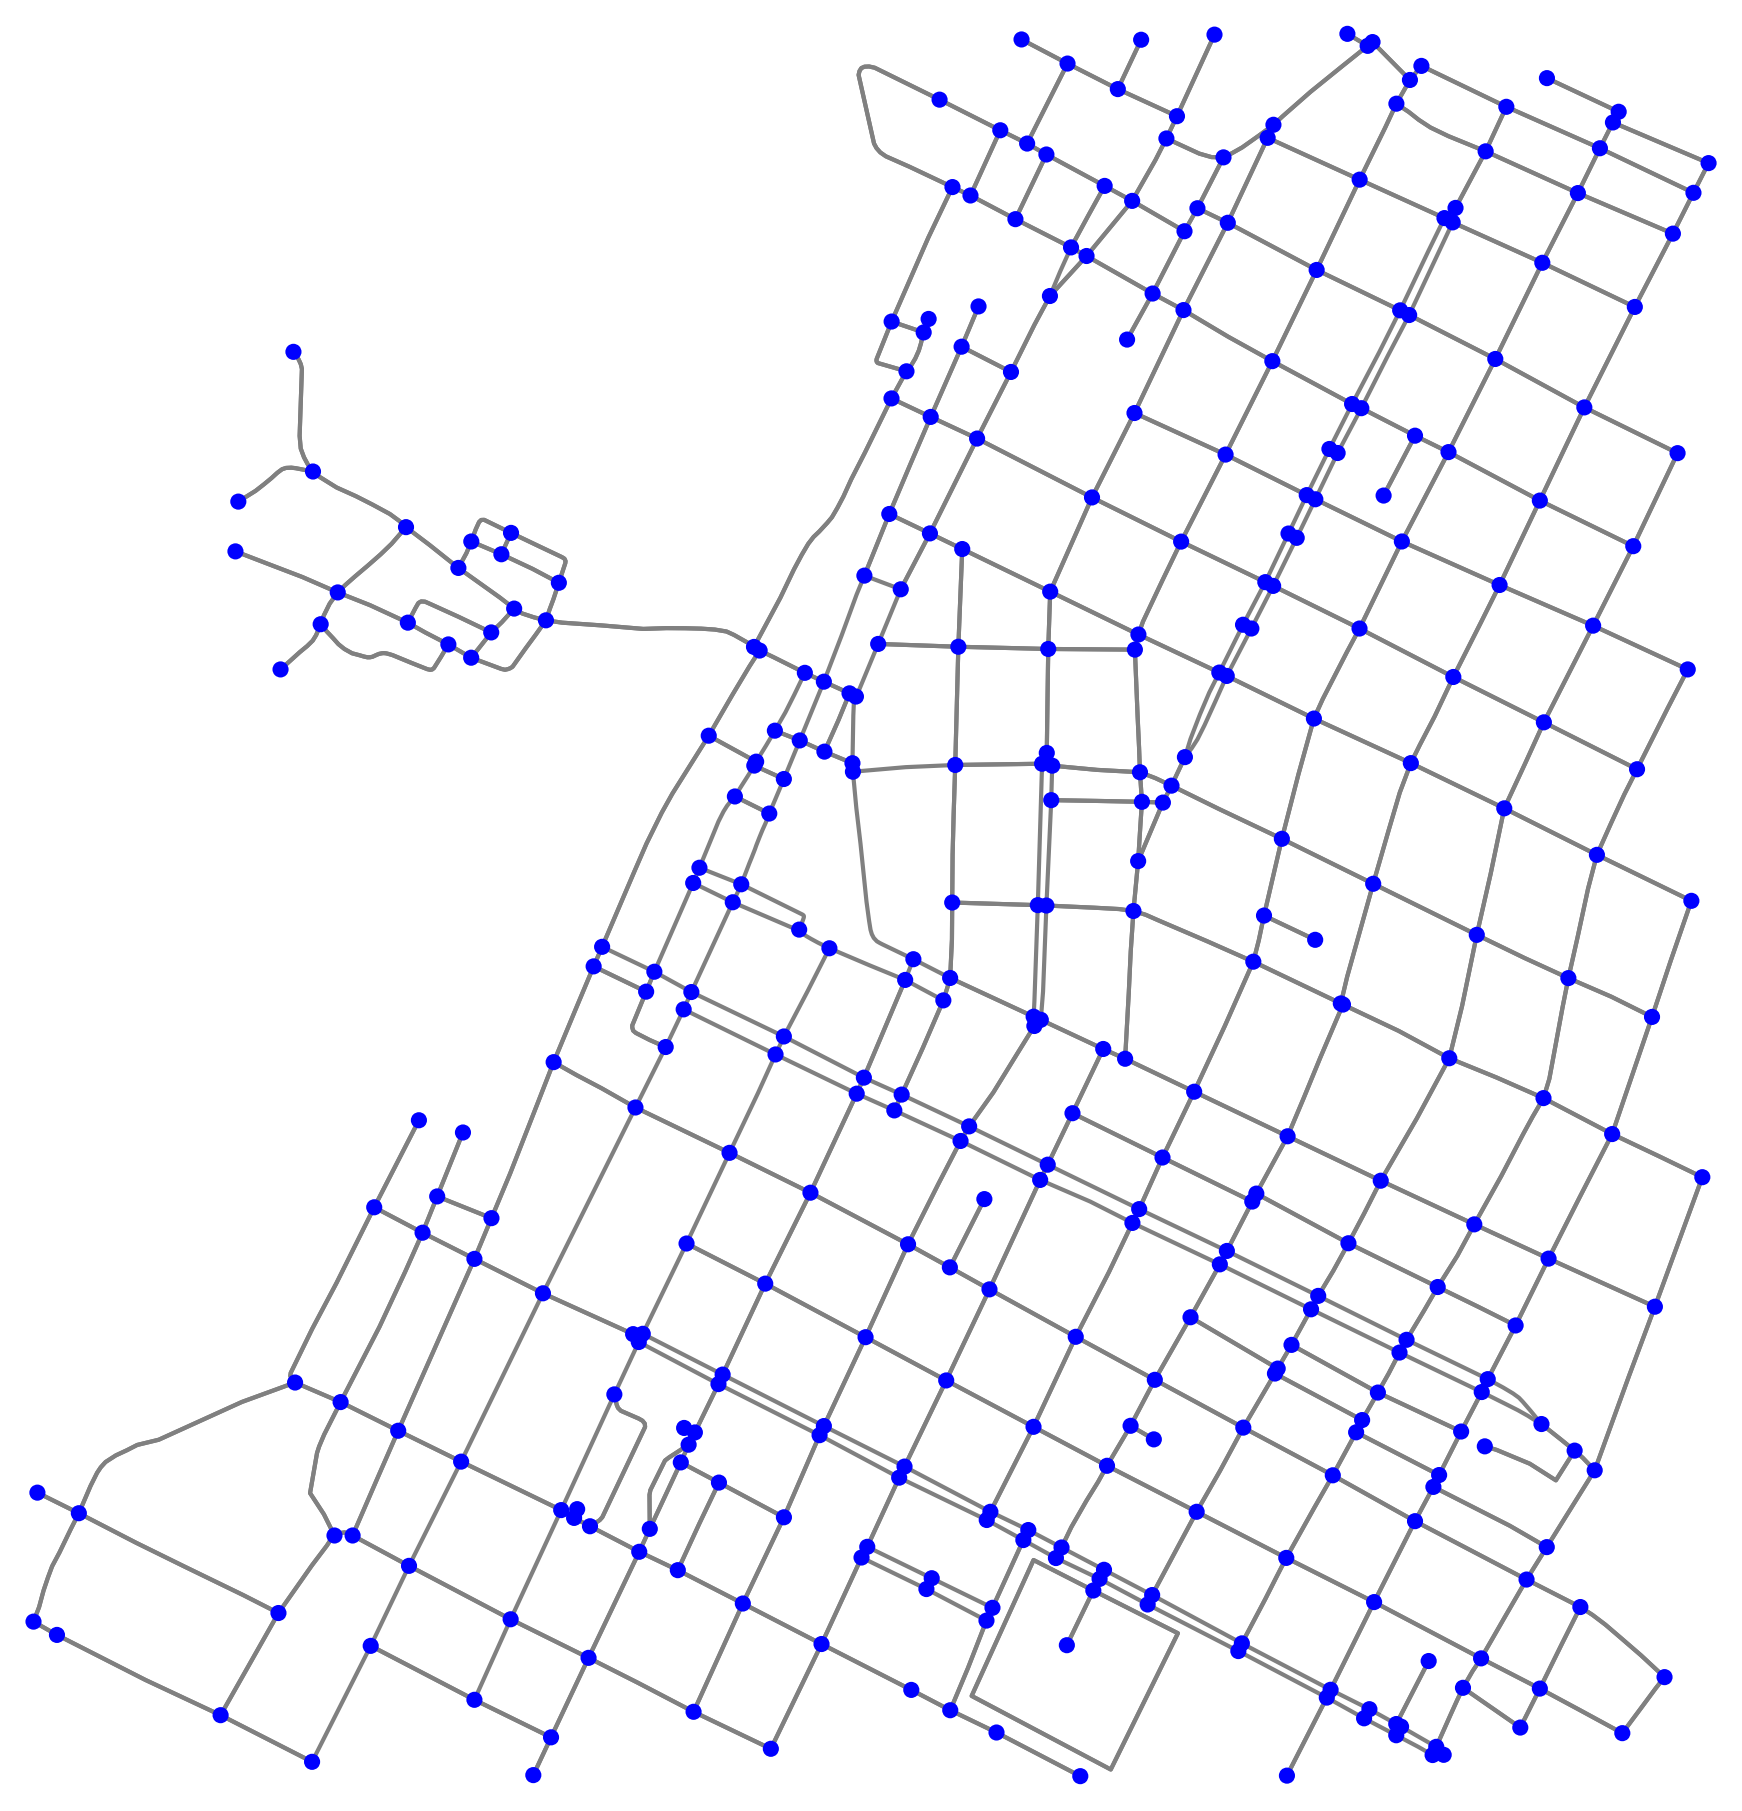
\includegraphics[width=7cm, height=6cm]{images/graph-limoeiro.png}}
	\end{minipage}
	\caption{\label{fig:graph-examples} Representation of the two cities used in the benchmark.}
\end{figure}


\begin{table}[h!]
	\centering
	\caption{Benchmark main characteristics.}
	\label{tab:real-instances}
	\begin{tabular}{lrrrrr}
		\hline
		\multicolumn{1}{c}{Instances}                                                &
		\multicolumn{1}{c}{$|V|$}                                                    &
		\multicolumn{1}{c}{$|A|$}                                                    &
		\multicolumn{1}{c}{$|B|$}                                                    &
		\multicolumn{1}{c}{\begin{tabular}[c]{@{}c@{}}Notified\\ Cases\end{tabular}} &
		\multicolumn{1}{c}{\begin{tabular}[c]{@{}c@{}}Blocks with\\ Cases (\%)\end{tabular}}                            \\ \hline
		AS-1000-2016                                                                 & 179  & 499  & 73  & 35   & 13.70 \\
		AS-1000-2017                                                                 & 179  & 499  & 73  & 194  & 36.99 \\
		AS-1000-2018                                                                 & 179  & 499  & 73  & 196  & 36.99 \\
		AS-1000-2019                                                                 & 179  & 499  & 73  & 196  & 36.99 \\
		AS-1000-2020                                                                 & 179  & 499  & 73  & 204  & 36.99 \\
		AS-1000-2021                                                                 & 179  & 499  & 73  & 218  & 36.99 \\ \hline
		AS-2000-2016                                                                 & 253  & 684  & 88  & 26   & 9.09  \\
		AS-2000-2017                                                                 & 253  & 684  & 88  & 174  & 29.55 \\
		AS-2000-2018                                                                 & 253  & 684  & 88  & 174  & 29.55 \\
		AS-2000-2019                                                                 & 253  & 684  & 88  & 174  & 29.55 \\
		AS-2000-2020                                                                 & 253  & 684  & 88  & 181  & 29.55 \\
		AS-2000-2021                                                                 & 253  & 684  & 88  & 195  & 30.68 \\ \hline
		AS-3000-2016                                                                 & 353  & 946  & 114 & 33   & 8.77  \\
		AS-3000-2017                                                                 & 353  & 946  & 114 & 198  & 24.56 \\
		AS-3000-2018                                                                 & 353  & 946  & 114 & 198  & 24.56 \\
		AS-3000-2019                                                                 & 353  & 946  & 114 & 198  & 24.56 \\
		AS-3000-2020                                                                 & 353  & 946  & 114 & 206  & 24.56 \\
		AS-3000-2021                                                                 & 353  & 946  & 114 & 225  & 24.56 \\ \hline
		LN-1000-2015                                                                 & 372  & 1063 & 152 & 18   & 7.89  \\
		LN-1000-2016                                                                 & 372  & 1063 & 152 & 26   & 10.53 \\
		LN-1000-2017                                                                 & 372  & 1063 & 152 & 50   & 17.11 \\
		LN-1000-2018                                                                 & 372  & 1063 & 152 & 51   & 17.11 \\
		LN-1000-2019                                                                 & 372  & 1063 & 152 & 66   & 20.39 \\
		LN-1000-2020                                                                 & 372  & 1063 & 152 & 163  & 29.61 \\
		LN-1000-2021                                                                 & 372  & 1063 & 152 & 168  & 31.58 \\ \hline
		LN-2000-2015                                                                 & 980  & 2866 & 443 & 174  & 6.77  \\
		LN-2000-2016                                                                 & 980  & 2866 & 443 & 337  & 9.03  \\
		LN-2000-2017                                                                 & 980  & 2866 & 443 & 527  & 12.19 \\
		LN-2000-2018                                                                 & 980  & 2866 & 443 & 543  & 12.64 \\
		LN-2000-2019                                                                 & 980  & 2866 & 443 & 875  & 14.22 \\
		LN-2000-2020                                                                 & 980  & 2866 & 443 & 2183 & 20.99 \\
		LN-2000-2021                                                                 & 980  & 2866 & 443 & 2316 & 21.67 \\ \hline
		LN-3000-2015                                                                 & 1212 & 3497 & 517 & 169  & 5.22  \\
		LN-3000-2016                                                                 & 1212 & 3497 & 517 & 336  & 7.54  \\
		LN-3000-2017                                                                 & 1212 & 3497 & 517 & 519  & 10.83 \\
		LN-3000-2018                                                                 & 1212 & 3497 & 517 & 533  & 11.03 \\
		LN-3000-2019                                                                 & 1212 & 3497 & 517 & 860  & 12.38 \\
		LN-3000-2020                                                                 & 1212 & 3497 & 517 & 2176 & 18.96 \\
		LN-3000-2021                                                                 & 1212 & 3497 & 517 & 2315 & 19.92 \\ \hline
	\end{tabular}%
\end{table}



